\documentclass{article}  % Define la clase del documento.

% Paquetes de idioma y codificación
\usepackage[utf8]{inputenc}
\usepackage[T1]{fontenc}
%\usepackage[spanish]{babel}  % Ajusta el idioma del documento a español.
\usepackage{tabularx}  % Permite la creación de tablas con ancho ajustable.

\usepackage{caption}
\usepackage{subcaption}

% Paquete de geometría para configurar márgenes y tamaño de papel
\usepackage[letterpaper, margin=3cm]{geometry}

\usepackage[english]{babel}
\addto\captionsspanish{%
  \renewcommand{\tablename}{Table}%
  \renewcommand{\figurename}{Figure}%
}

% Paquetes de tipografía
\usepackage{mathptmx}    % Usa Times New Roman como fuente.
\usepackage{microtype}   % Mejora la justificación del texto.

% Paquetes para manejo de colores y gráficos
\usepackage{xcolor}      % Define y utiliza colores.
\usepackage{graphicx}    % Permite la inserción de imágenes.
\usepackage{tikz}        % Creación de gráficos vectoriales.

% Configuración de enlaces y referencias cruzadas
\usepackage{hyperref}
\hypersetup{
    colorlinks   = true,
    linkcolor    = darkblue,
    citecolor    = black,
    filecolor    = blue,
    urlcolor     = blue
}

\usepackage{media9} % Permite la inserción de multimedia.

% Paquetes para la mejora visual de tablas y figuras
\usepackage{booktabs}    % Para tablas de alta calidad.
\usepackage{float}       % Controla la posición de figuras y tablas.

% Paquete para la personalización de códigos fuente
\usepackage{listings}
\lstset{
    literate=
    {á}{{\'a}}1 {é}{{\'e}}1 {í}{{\'i}}1 {ó}{{\'o}}1 {ú}{{\'u}}1
    {Á}{{\'A}}1 {É}{{\'E}}1 {Í}{{\'I}}1 {Ó}{{\'O}}1 {Ú}{{\'U}}1
    {ñ}{{\~n}}1 {Ñ}{{\~N}}1 {ü}{{\"u}}1 {Ü}{{\"U}}1,
    backgroundcolor=\color{backcolour},
    commentstyle=\color{codegreen},
    keywordstyle=\color{codepurple},
    numberstyle=\tiny\color{codegray},
    stringstyle=\color{red},
    basicstyle=\ttfamily\small,
    breakatwhitespace=false,
    breaklines=true,
    captionpos=b,
    keepspaces=true,
    numbers=left,
    numbersep=5pt,
    showspaces=false,
    showstringspaces=false,
    showtabs=false,
    tabsize=2,
    language=TeX,
    morecomment=[l]\#,
    frame=single,
    rulecolor=\color{black}
}

% Definición de colores al estilo Visual Studio Code
\definecolor{darkblue}{rgb}{0.0, 0.0, 0.55}  % Enlaces
\definecolor{codegreen}{rgb}{0.25, 0.49, 0.48}  % Comentarios
\definecolor{codegray}{rgb}{0.5, 0.5, 0.5}  % Números y anotaciones
\definecolor{codepurple}{rgb}{0.58, 0, 0.82}  % Palabras clave
\definecolor{backcolour}{rgb}{0.95, 0.95, 0.92}  % Fondo de código

% Configuraciones de párrafo y matemáticas
\usepackage{amsmath}
\usepackage{parskip}    % Espaciado entre párrafos.
\usepackage{ragged2e}   % Justificación mejorada.
\usepackage{multicol}

% Configuración de secciones y encabezados
\usepackage{titlesec}
\titleclass{\part}{top} % Make part like a class
\titleformat{\part}[display]
  {\normalfont\huge\bfseries\centering}{\thepart}{40pt}{\Huge}
\titlespacing*{\part}{0pt}{-60pt}{10pt}
\titleformat{\part}
  {\normalfont\huge\bfseries}{}{0pt}{}

% Asegúrate de usar esto para mantener el estilo en las páginas de las partes
\titleformat{\part}[display]
  {\normalfont\huge\bfseries}{}{0pt}{}
  [\thispagestyle{fancy}] % Aplica el estilo fancy a las páginas de las partes

% Configuración de encabezados y pies de página personalizados
\usepackage{fancyhdr}
\pagestyle{fancy}
\fancyhf{}
\fancyhead[L]{\raisebox{0.20cm}{\textbf{Dynamics of structures}}}
\fancyhead[R]{\raisebox{0.1cm}{
\includegraphics[width=0.25\linewidth]{LOGO_UNIVERSIDAD.jpg}}}
\fancyhead[C]{\rule{\textwidth}{0.6pt}}
\fancyfoot[C]{\rule{\textwidth}{0.6pt}}
\fancyfoot[R]{\raisebox{-1.5\baselineskip}{\thepage}}
\renewcommand{\headrulewidth}{0pt}
\renewcommand{\footrulewidth}{0pt}

% Configuración avanzada de geometría
\geometry{
  top=3.5cm, % Aumenta el espacio en la parte superior para subir el encabezado
  bottom=2.5cm,
  headheight=2.5cm % Aumenta la altura del encabezado si es necesario
}

% Configuracion de bibliografia
\usepackage{natbib}
\bibliographystyle{unsrtnat}  % Puedes cambiarlo por `unsrtnat`, `abbrvnat`, etc.

\begin{document}
%----------------------------------------------------------------------------------------
% PORTADA
%----------------------------------------------------------------------------------------
\begin{titlepage}%Inicio de la carátula, solo modificar los datos necesarios
\newcommand{\HRule}{\rule{\linewidth}{0.5mm}} 
\center 
%----------------------------------------------------------------------------------------
%	ENCABEZADO
%----------------------------------------------------------------------------------------

\includegraphics[width=10cm]{LOGO_UNIVERSIDAD.jpg}\\ % Si esta plantilla se copio correctamente, va a llevar la imagen del logo de la facultad.OBS: Es necesario incluir el paquete: graphicx
\vspace{3cm}
%----------------------------------------------------------------------------------------
%	SECCION DEL TITULO
%----------------------------------------------------------------------------------------
\HRule \\[0.4cm]
{ \huge \bfseries Dynamics of structures}\\[0.4cm] % Titulo del documento
{ \huge \bfseries Laboratory 2: Multiple Degrees of Freedom System}\\[0.4cm] % Titulo del documento
\HRule \\[1.5cm]
 \vspace{4cm}
%----------------------------------------------------------------------------------------
%	SECCION DEL AUTOR
%----------------------------------------------------------------------------------------
\begin{flushright}
  { \textbf{Professor:}\\
  Francisco Hernandez\\
  \textbf{Assistance:}\\
  Gastón Parra\\
  \textbf{Students:} \\
  Bernardo Caprile\\
  Pedro Valenzuela\\
  Felipe Vicencio\\
  Lukas Wolff\\
}
\end{flushright}
\vspace{1cm}
%----------------------------------------------------------------------------------------
%	SECCION DE LA FECHA
%----------------------------------------------------------------------------------------
{\large \textbf{\today}}\\[2cm] % El comando \today coloca la fecha del dia, y esto se actualiza con cada compilacion, en caso de querer tener una fecha estatica, reemplazar el \today por la fecha deseada
\end{titlepage}

\newpage
\thispagestyle{empty} % Deshabilita el número de página en la página del índice

%----------------------------------------------------------------------------------------
%  INDICE
%----------------------------------------------------------------------------------------
%\newpage
%\thispagestyle{empty} % Deshabilita el número de página en la página del índice
%\tableofcontents
%\thispagestyle{plain} % Deshabilita el encabezado en la página del índice
%\thispagestyle{empty} % Deshabilita el número de página en la página del índice
%\newpage

%\newpage
%\thispagestyle{empty}
%\listoffigures 
%\thispagestyle{plain} % Deshabilita el encabezado en la página del índice %
%\thispagestyle{empty}
\newpage
%----------------------------------------------------------------------------------------
%ACÁ EMPIEZA EL INFORME
\setcounter{page}{1}
%----------------------------------------------------------------------------------------

\section{Introduction}

Understanding the dynamic behavior of real-world structures requires the analysis of systems with multiple degrees of freedom (MDOF). Unlike single degree of freedom (SDOF) models, which offer only a simplified representation, MDOF systems provide a more realistic framework for simulating buildings, bridges, and mechanical structures subjected to dynamic loads such as wind, traffic, and earthquakes. These systems are characterized by multiple natural frequencies and associated mode shapes, each contributing uniquely to the overall structural response.

\begin{figure}[h]
    \centering
    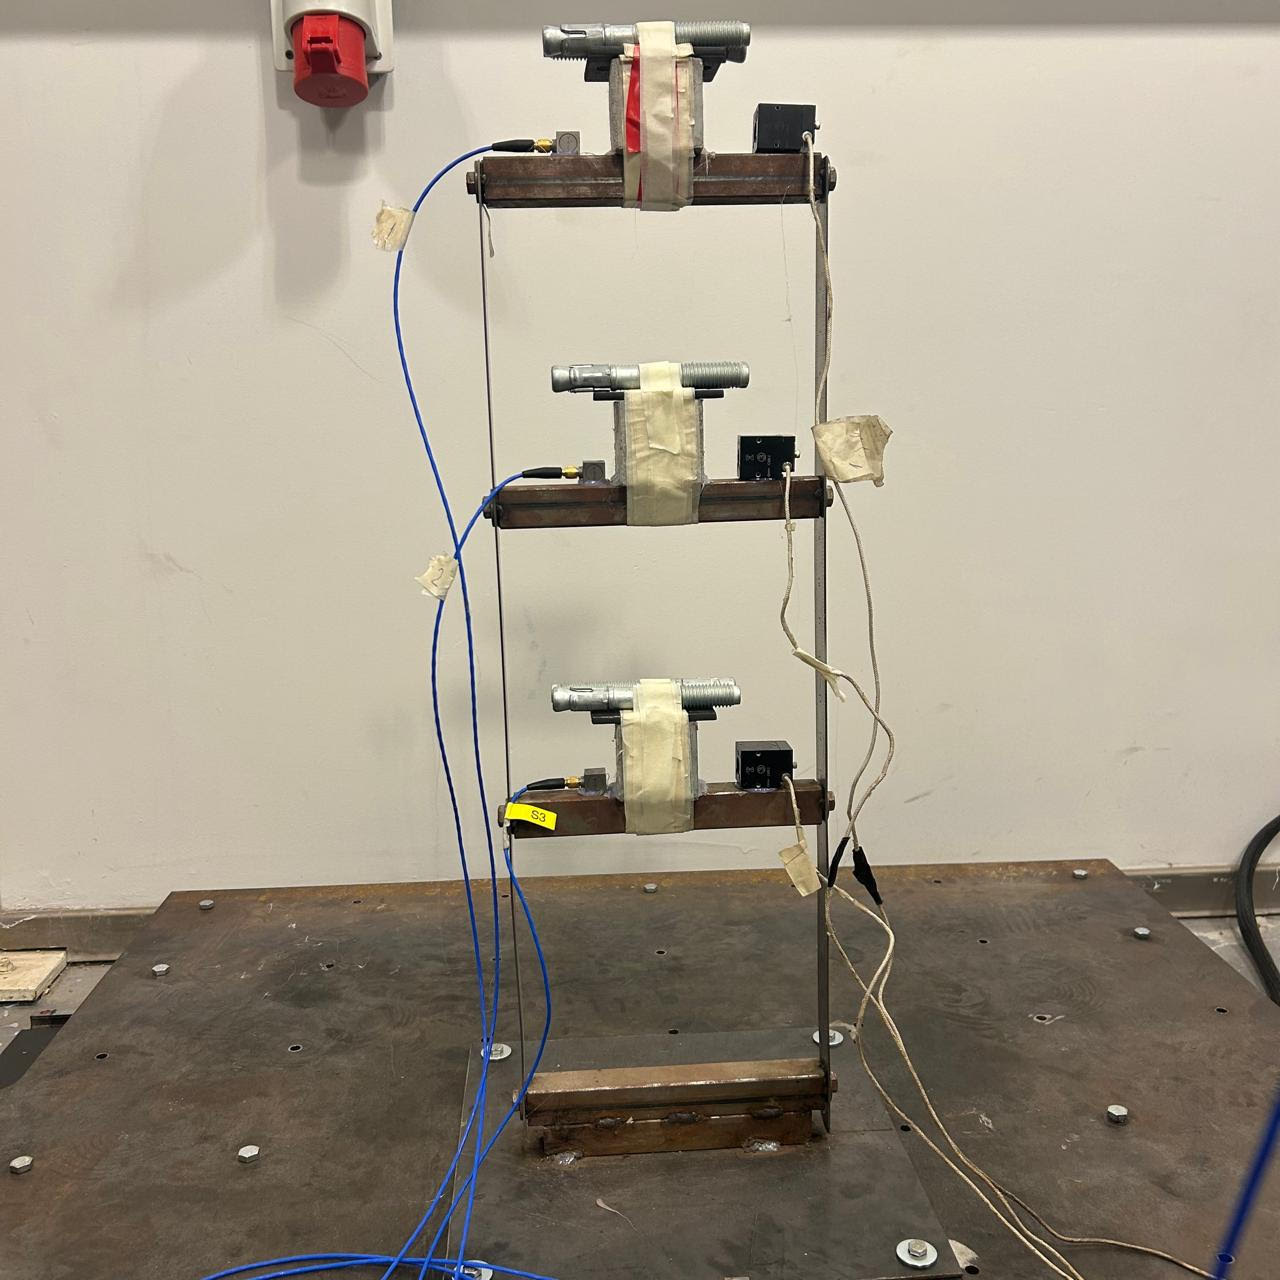
\includegraphics[width=0.5\textwidth]{GRAFICOS/model.jpg}
    \caption{Representation of an MDOF structural model}
    \label{fig:sdof_vs_mdof}
\end{figure}

This laboratory experiment focuses on the dynamic analysis of an MDOF system subjected to various excitation conditions. The primary objectives are:
\begin{itemize}
    \item To identify the natural frequencies and corresponding mode shapes of a 3-degree-of-freedom structure through analytical and experimental methods.
    \item To evaluate the system’s response under free vibration (pullback tests) and harmonic excitation, including the influence of damping and resonance.
    \item To analyze the seismic response of the system under two real earthquake records (Kobe and Concepción), using both analytical simulations and experimental data.
\end{itemize}

This comprehensive study builds upon the theoretical foundations of SDOF systems and extends them to more complex configurations. It provides critical insights into modal analysis, dynamic amplification, and the effect of damping essential concepts for the safe and effective design of real engineering structures subjected to dynamic loads.

\newpage

\section{Theoretical Background}

\subsection{Natural Frequency}
The natural frequency of a system is the rate at which the body oscillates when it is disturbed without any damping or external forces acting on it. This parameter is crucial in understanding the dynamic behavior of structures, as it determines how the system will respond to external excitations. The natural frequency can be calculated using the following formula:
\begin{equation}
\omega_n = \sqrt{\frac{k}{m}}
\end{equation}
Where:
\begin{itemize}
  \item $\omega_n$ = natural frequency (rad/s)
  \item $k$ = stiffness of the system (N/m)
  \item $m$ = mass of the system (kg)
\end{itemize}

One of the important aspects of the natural frequency is that it is inversely proportional to the mass of the system. This means that as the mass increases, the natural frequency decreases, and vice versa. This relationship is crucial in designing structures to ensure they can withstand dynamic loads without resonating at their natural frequency.

\subsection{Damping Ratio}
The damping ratio is a parameter that has the effect of reducing the oscillations of a system over time. In physical systems, damping is caused by energy dissipation mechanisms such as friction, air resistance or dampers. The damping ratio is defined as the ratio of the actual damping to the critical damping, and it can be calculated using the following formula:
\begin{equation}
\beta = \frac{c}{2\sqrt{mk}}
\end{equation}
Where:
\begin{itemize}
  \item $\beta$ = damping ratio (dimensionless)
  \item $c$ = damping coefficient (N.s/m)
  \item $k$ = stiffness of the system (N/m)
  \item $m$ = mass of the system (kg)
\end{itemize}

\subsection{Logarithmic Decrement}
The logarithmic decrement is a measure of the rate at which the amplitude of oscillations decreases over time in a damped system. It is defined as the natural logarithm of the ratio of two successive amplitudes, and it can be calculated using the following formula:

\begin{equation}
\delta = \frac{1}{n} \ln \left( \frac{x_0}{x_n} \right)
\end{equation}
Where:
\begin{itemize}
  \item $\delta$ = logarithmic decrement (dimensionless)
  \item $x_0$ = amplitude of the first oscillation (m)
  \item $x_n$ = amplitude of the n-th oscillation (m)
  \item $n$ = number of oscillations (dimensionless)
\end{itemize}

With this parameter, we can determine the damping ratio of the system using the following formula:

\begin{equation}
\beta = \frac{\delta}{\sqrt{4\pi^2 + \delta^2}}
\label{eq:log_dec}
\end{equation}
Where:
\begin{itemize}
  \item $\delta$ = logarithmic decrement (dimensionless)
  \item $\beta$ = damping ratio (dimensionless)
\end{itemize}

\subsection{Harmonic base excitation}
The harmonic base excitation is a phenomenon that occurs when a system is subjected to a periodic force at its base. This type of excitation is key in understanding the dynamic behavior of structures, due to every structure suffers from this type of excitation. 

\subsection{Transmissibility}
Transmissibility is a measure of how much the input motion is transmitted to the output of a system. It is defined as the ratio of the output response to the input response, and it can be calculated using the following formula:
\begin{equation}
TR = \frac{\ddot{X}}{\ddot{X_g}} = \sqrt{\frac{1+(2 \beta (\bar{\omega}/\omega_n)^2}{(1 - \frac{\bar{\omega}^2}{\omega_n^2})^2 + (2\beta\frac{\bar{\omega}}{\omega_n})^2}} 
\label{eq:transmissibility}
\end{equation}
Where:
\begin{itemize}
  \item $TR$ = transmissibility (dimensionless)
  \item $\ddot{X_g}$ = output acceleration (m/s$^2$) (acceleration of the base) 
  \item $\ddot{X}$ = input acceleration (m/s$^2$) (acceleration of the mass)
  \item $\bar{\omega}$ = frequency of the input motion (rad/s)
  \item $\omega_n$ = natural frequency of the system (rad/s)
  \item $\beta$ = damping ratio (dimensionless)
\end{itemize}

Due to the transmissibility, if the excitation frequency is much smaller than the natural frequency of the system ($\bar{\omega} < \omega_n$), the transmissibility is close to 1, which means that the input motion is transmitted to the output with little amplification. On the other hand, if the excitation frequency is larger than the natural frequency of the system ($\bar{\omega} > \omega_n$), the transmissibility is close to 0, which means that the input motion is transmitted to the output with null amplification. Finally, if the excitation frequency is equal to the natural frequency of the system ($\bar{\omega} = \omega_n$), the transmissibility is infinite, which means that the input motion is transmitted to the output with a high amplification. This phenomenon is known as resonance.

\subsection{Resonance}
Resonance is a phenomenon that occurs when the frequency of an external force matches the natural frequency of a system:

$$\omega_n = \bar{\omega}$$

For an undamped system the factor of amplification is infinite, which means that the system will oscillate indefinitely with increasing amplitude. In real systems, damping reduces the maximum amplitude of oscillations, but resonance can still lead to significant increases in amplitude. This means, if the resonance is not controlled, it can cause structural damage or failure. 
\subsection{Mass Matrix and Stiffness Matrix}
In multi-degree-of-freedom (MDOF) systems, the dynamic behavior is governed by the equation of motion:

\begin{equation}
\mathbf{M} \ddot{\mathbf{X}}(t) + \mathbf{C} \dot{\mathbf{X}}(t) + \mathbf{K} \mathbf{X}(t) = \mathbf{F}(t)
\end{equation}

Where:
\begin{itemize}
  \item $\mathbf{M}$ = mass matrix (kg)
  \item $\mathbf{C}$ = damping matrix (kg/s)
  \item $\mathbf{K}$ = stiffness matrix (N/m)
  \item $\mathbf{X}(t)$ = displacement vector
  \item $\mathbf{F}(t)$ = external force vector
\end{itemize}

The mass matrix $\mathbf{M}$ is a diagonal matrix in most lumped mass models, where each diagonal term represents the mass associated with a degree of freedom. The stiffness matrix $\mathbf{K}$ defines the relationship between nodal displacements and restoring forces in the system. Its entries depend on the stiffness properties of structural members.


Where:
\begin{itemize}
  \item $\omega$ = natural angular frequency (rad/s)
  \item $\boldsymbol{\phi}$ = mode shape vector (eigenvector)
\end{itemize}

Each mode shape is associated with a unique natural frequency, and the set of mode shapes forms a complete, linearly independent basis for the system’s motion.

\subsection{Eigenvalues and Eigenvectors}
Solving the eigenvalue problem yields:
\begin{itemize}
  \item \textbf{Eigenvalues} $\lambda_i = \omega_i^2$, which represent the squared natural frequencies of the system.
  \item \textbf{Eigenvectors} $\boldsymbol{\phi}_i$, which represent the mode shapes corresponding to each frequency.
\end{itemize}

The eigenvalue problem for free vibration (undamped) systems is:

\begin{equation}
\mathbf{K} \boldsymbol{\phi}_i = \lambda_i \mathbf{M} \boldsymbol{\phi}_i
\end{equation}

By taking the square root of the eigenvalues, we obtain the natural frequencies $\omega_i = \sqrt{\lambda_i}$. These values provide critical information about the dynamic response of the structure and are used to identify potential resonance conditions.

\subsection{Mode Shapes}
The mode shapes (or eigenvectors) of a system represent the relative displacements of each degree of freedom during free vibration at a specific natural frequency. They are determined by solving the eigenvalue problem of the undamped system:

\begin{equation}
\left( \mathbf{K} - \omega^2 \mathbf{M} \right) \boldsymbol{\phi} = \mathbf{0}
\end{equation}




\newpage
\section{Structure Description}

The structure analyzed in this laboratory corresponds to a three-degree-of-freedom (3DOF) system subjected to free vibration. It consists of three vertically aligned masses connected by steel beams that provide bending stiffness. Each mass is allowed to move in the vertical direction, and the structure mimics a simplified building model with lumped masses and flexible connections. The dynamic response was captured using accelerometers placed on each mass.

\textbf{Masses:} \\
The total mass of the system is concentrated in three rigid blocks, each formed by stacked steel components and instrumentation. Additionally, the self-weight of the connecting beams is included in the equivalent mass at each level. 

The structure follows the assumption that masses are not tributary: each degree of freedom is associated with a single lumped mass, which receives half the weight of the beams above and half of those below. Therefore, the equivalent lumped masses for each degree of freedom are:

\begin{itemize}
    \item $m_1 = 0.555 + 0.26 + 4 \times \frac{0.075}{6} = 0.829$ kg
    \item $m_2 = 0.553 + 0.26 + 8 \times \frac{0.075}{6} = 0.993$ kg
    \item $m_3 = 0.691 + 0.26 + 8 \times \frac{0.075}{6} = 1.131$ kg
\end{itemize}

These values include half of the mass of each adjacent beam, distributed based on the position of each mass in the structure.

The mass matrix $\mathbf{M}$ (in Tonf·s$^2$/m) is:

\[
\mathbf{M} = \begin{bmatrix}
8.45 \times 10^{-5} & 0 & 0 \\
0 & 1.01 \times 10^{-4} & 0 \\
0 & 0 & 1.15 \times 10^{-4}
\end{bmatrix}
\]

\textbf{Stiffness:} \\
The stiffness of each level is governed by the flexural stiffness of the steel beams, modeled as fixed-fixed beams. Each column consists of two metallic rulers (steel strips) working in parallel, which increases the total stiffness of each connection.

The stiffness of a single beam is calculated as:

\[
k_{\text{single}} = \frac{48EI}{L^3}
\]

Since each connection is composed of two identical rulers acting in parallel, the total stiffness per level becomes:

\[
k_i = 2 \times k_{\text{single}} = \frac{96EI}{L^3}
\]

Where:
\begin{itemize}
    \item $E = 200\,\text{GPa}$ is the Young's modulus of steel,
    \item $I = \frac{1}{12} b h^3$ is the second moment of area,
    \item $L = 0.6/3 = 0.2\,\text{m}$ is the span of each beam.
\end{itemize}

With this, the stiffness per level is:

\[
k_i = \frac{96EI}{L^3} \approx 110{,}371.4\, \text{Tonf/m}
\]

The global stiffness matrix $\mathbf{K}$ (in Tonf/m) is:

\[
\mathbf{K} = \begin{bmatrix}
110371.4 & -110371.4 & 0 \\
-110371.4 & 220742.8 & -110371.4 \\
0 & -110371.4 & 220742.8
\end{bmatrix}
\]

\textbf{Natural Frequencies:} \\
The natural frequencies of the system were computed using the eigenvalue problem $\mathbf{K}\phi = \omega^2 \mathbf{M} \phi$. The eigenvalues were obtained, and then the natural frequencies were calculated as:

\[
\omega_n = \sqrt{\lambda_n}, \quad f_n = \frac{\omega_n}{2\pi}
\]

The computed natural frequencies are:

\[
\omega_1 = 14.06\,\text{rad/s}, \quad \omega_2 = 37.96\,\text{rad/s}, \quad \omega_3 = 55.57\,\text{rad/s}
\]
\[
f_1 = 2.24\,\text{Hz}, \quad f_2 = 6.04\,\text{Hz}, \quad f_3 = 8.84\,\text{Hz}
\]

\subsection*{Theoretical Mode Shapes}

The theoretical vibration modes of the 3DOF system are shown below. These represent the deformation patterns associated with each natural frequency computed from the analytical model.

\begin{figure}[H]
    \centering
    \begin{minipage}[b]{0.32\textwidth}
        \centering
        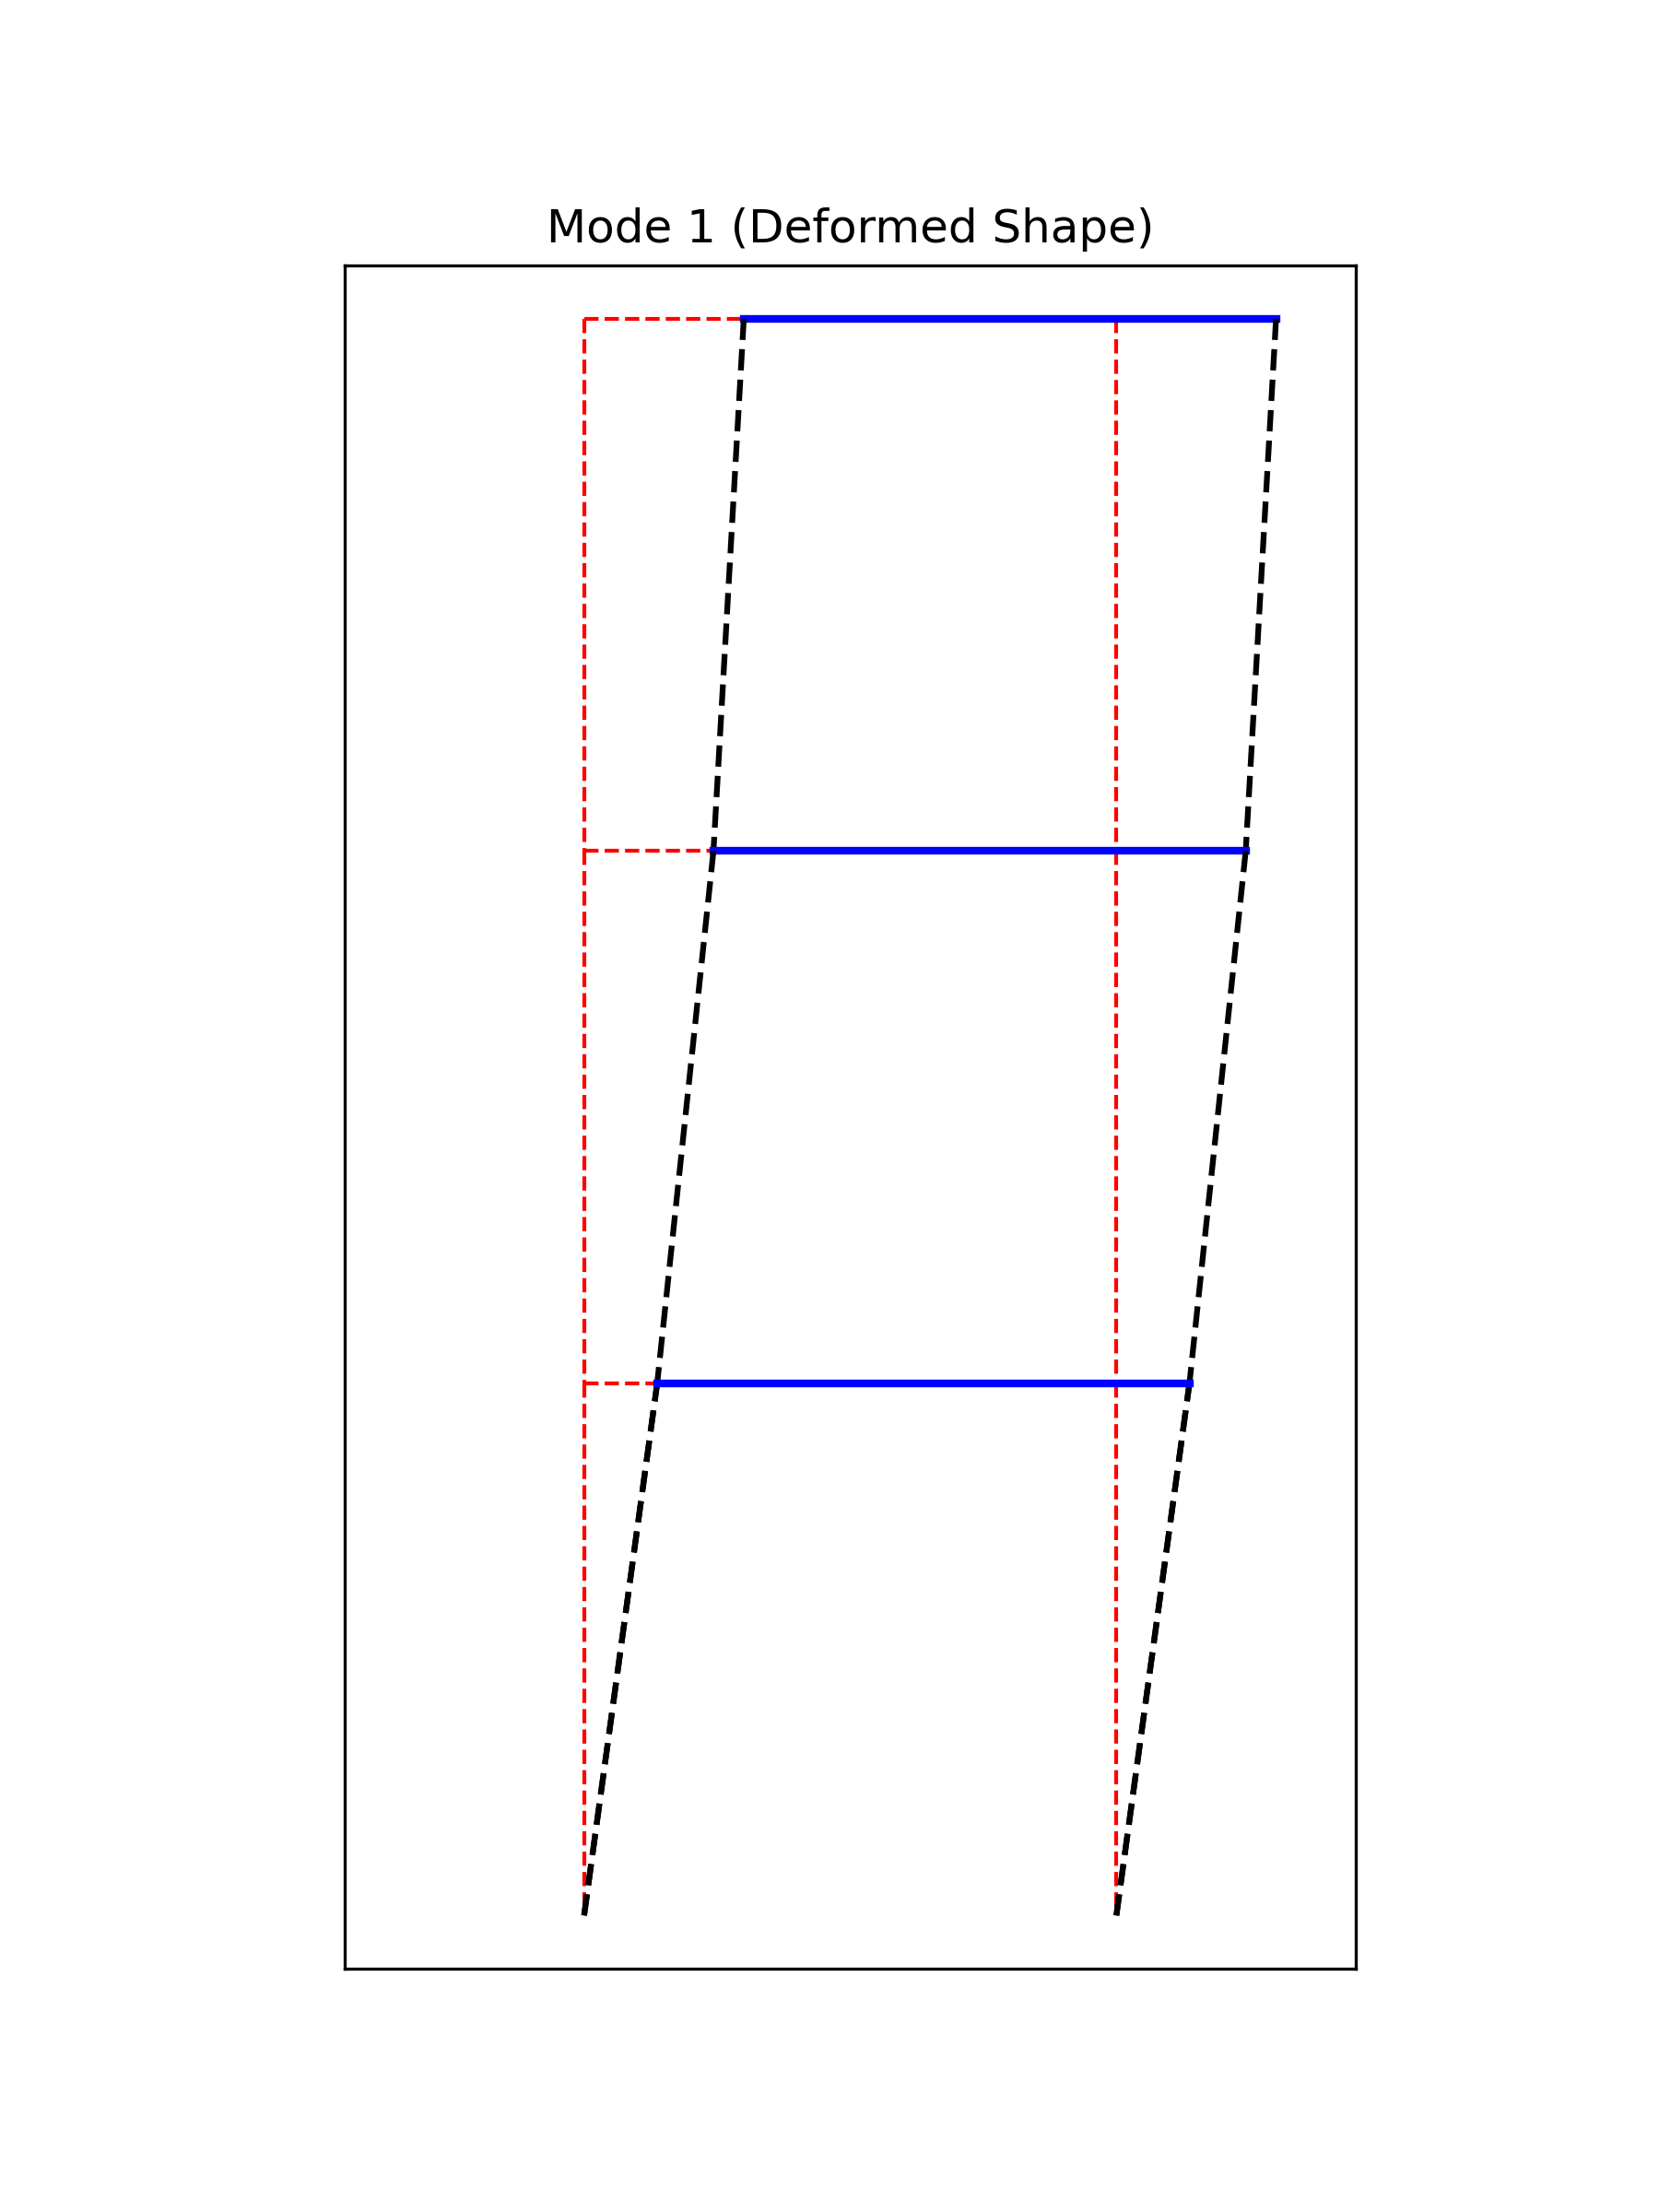
\includegraphics[width=\textwidth]{GRAFICOS/Modo_Estructura_1.png}
        \caption*{Mode 1}
    \end{minipage}
    \hfill
    \begin{minipage}[b]{0.32\textwidth}
        \centering
        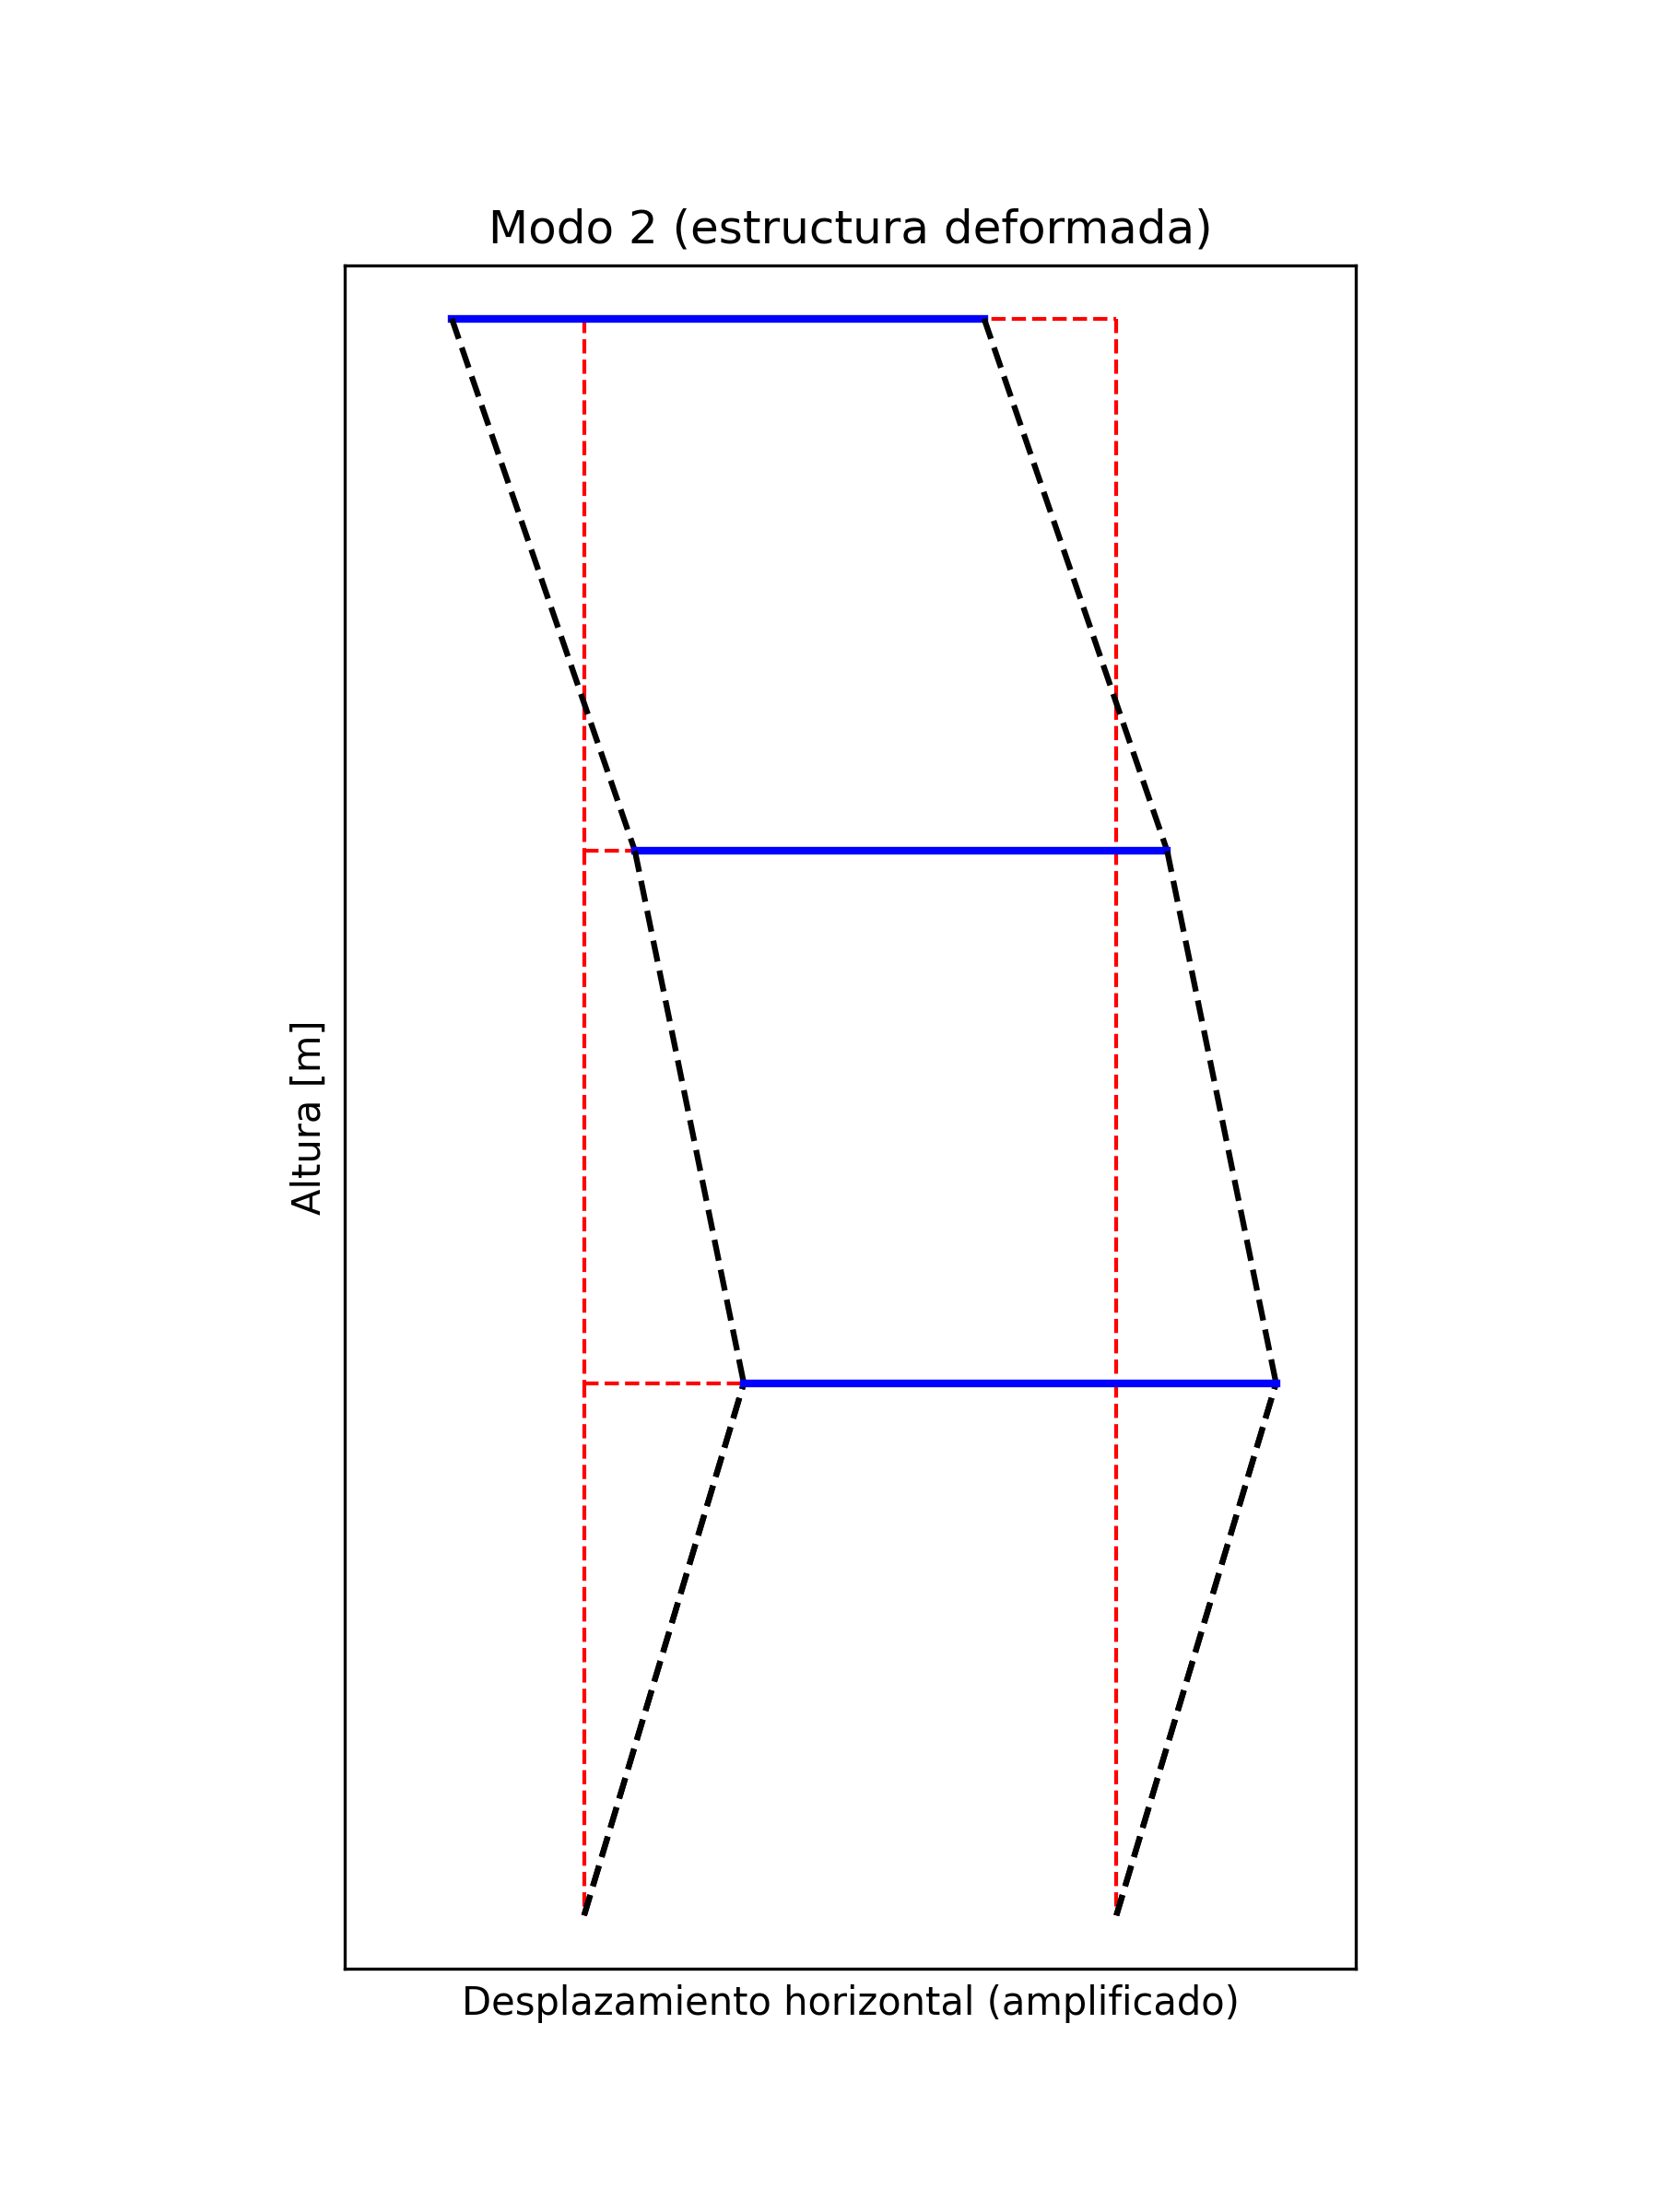
\includegraphics[width=\textwidth]{GRAFICOS/Modo_Estructura_2.png}
        \caption*{Mode 2}
    \end{minipage}
    \hfill
    \begin{minipage}[b]{0.32\textwidth}
        \centering
        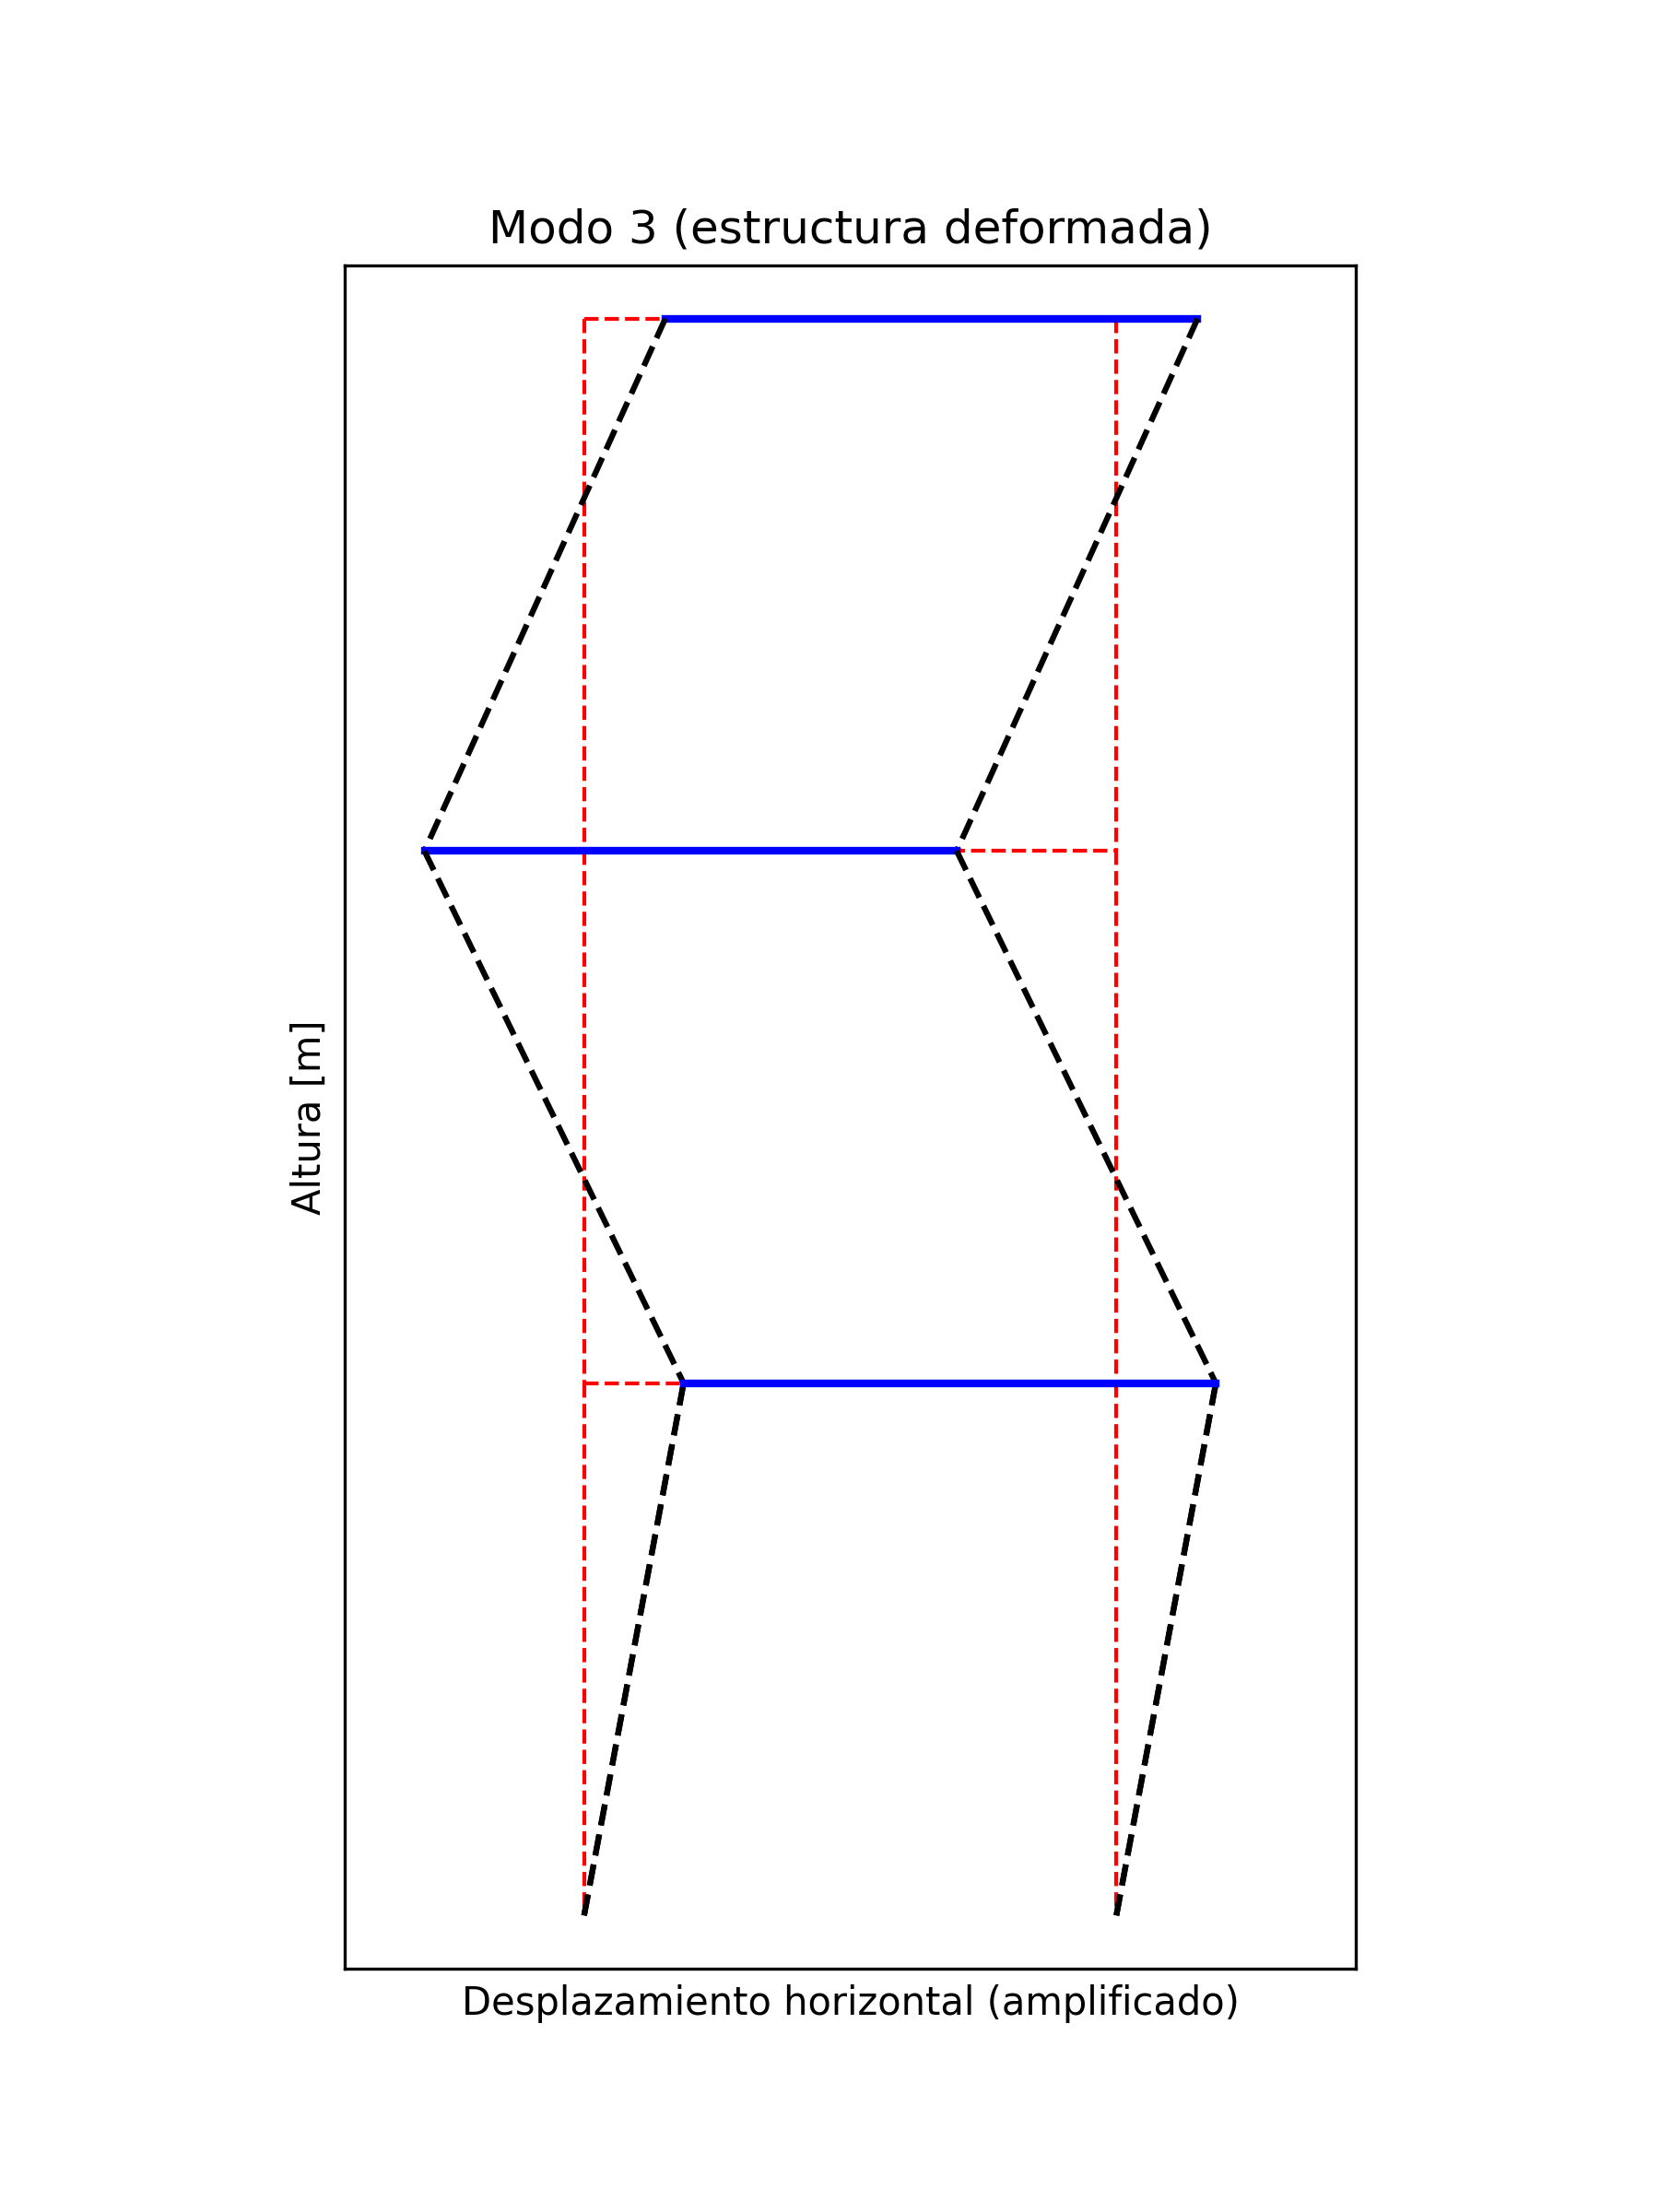
\includegraphics[width=\textwidth]{GRAFICOS/Modo_Estructura_3.png}
        \caption*{Mode 3}
    \end{minipage}
    \caption{Theoretical mode shapes of the 3DOF system.}
    \label{fig:mode_shapes}
\end{figure}

\newpage
\section{Instrumentation Details} 

\subsection{Endevco 44A16 Accelerometer}

The Endevco model 44A16 accelerometer is a triaxial IEPE (Integrated Electronics Piezo-Electric) sensor, designed for general-purpose vibration measurement applications, such as the dynamic analysis of the SDOF structure carried out in this laboratory. 

This model has a sensitivity of 100~mV/g and a measurement range of $\pm$50~g, which allows it to record significant accelerations without saturating the signal. In addition, it offers a useful frequency response range between 0.6~Hz and 5000~Hz depending on the axis, enabling it to capture the dynamic responses of various systems.


\subsection{QuantumX CX22B-W Data Acquisition System}

The QuantumX CX22B-W data acquisition system by HBM is a high-performance standalone data logger designed to capture, analyze, and store mechanical, electrical, or thermal variables without the need to be connected to an external computer. It is particularly useful for capturing data in structural analysis, as it can process data in real time and operate with multiple channels.

This device is equipped with a quad-core Intel Atom E3845 processor running at 1.9~GHz, 4~GB of RAM, and 240~GB of internal storage, in addition to a slot for a CFast card of up to 512~GB, which allows for extended data recording periods. It supports a maximum total sampling rate of 5~MS/s, making it capable of capturing high-frequency dynamic phenomena. Through its various input options, the system can integrate multiple types of sensors such as GPS units, cameras, and force sensors, among others.

For data analysis and visualization, the software \textit{Catman Easy} version 5.1.3 was used. This program enables the configuration of measurements and real-time data visualization, and allows automatic analysis such as the Fast Fourier Transform (FFT). In this case, acceleration responses were recorded and the FFT results were displayed every 5 seconds.


\subsection{TDG-250 KG Shaking Table}

The TDG-250 KG shaking table, manufactured by Teknik Destek Grubu, is a uniaxial seismic motion simulator designed for conducting structural dynamic tests in laboratory settings. Its maximum dynamic load capacity is 250~kg when applying an acceleration of 1~g, while for lighter loads of up to 100~kg, it can reach accelerations of up to $\pm$2~g. The table has a maximum stroke of $\pm$200~mm, a peak velocity of 800~mm/s, and an operational frequency of 15~Hz, making it suitable for a variety of dynamic input signals. Its displacement resolution is 0.0025~mm, providing high precision in motion control.

The system is driven by a servomotor and controlled via a closed-loop PID controller. It operates with a three-phase power supply of 3.3~kW at 380--480~V AC and 50 or 60~Hz.

The shaking table is operated using the \textit{Easy Test Shake Table} software, which allows the user to import and reproduce real earthquake records, such as those from Concepción, Chile or Kobe, Japan, as well as generate custom signals. The software supports various types of dynamic inputs, and during testing, it provides real-time visualization of acceleration, velocity, and displacement profiles, along with Fast Fourier Transform (FFT) results and response spectra.

\newpage
\section{Signal Processing}

Signal processing is carried out to prepare raw signals obtained from the sensors prior to analysis. This process includes two main techniques: detrending and digital filtering. Detrending involves removing constant components or linear trends from the signal, which may result from initial displacements, systematic errors, or very low-frequency noise. This technique allows the signal to be centered around zero, a necessary condition for computing parameters such as velocity and displacement.

Next, digital filtering is used to eliminate unwanted components from the signal, such as high-frequency noise or low-frequency elements that are not part of the structural response being analyzed.

Both techniques are implemented using the \textit{Catman Easy} software version 5.1.3, in conjunction with the QuantumX CX22B-W data acquisition system by HBM. This setup enables the recording and real-time visualization of the measured signals, as well as the application of digital processing during or after the test. Additionally, the software allows for the automatic visualization of the Fast Fourier Transform (FFT) at defined intervals, enabling the identification of dominant frequencies and the analysis of the dynamic behavior of the structure.


\newpage
\section{Laboratory Methodology}

The objective of this laboratory was to analyze the dynamic behavior of a multiple-degree-of-freedom (MDOF) structural system. To achieve this, a shaking table, acceleration sensors, and a data acquisition system were used.

First, a pull-back test was performed, which consisted of applying an initial lateral displacement to the structure and then releasing it to observe its free response. This test allowed the determination of the system’s natural periods and damping ratios through the analysis of the acceleration signal using the logarithmic decrement method. The Fast Fourier Transform (FFT) of the acceleration response was computed in real time every 5 seconds using the Catman Easy software (version 5.1.3).

Subsequently, a harmonic loading test was conducted, in which the shaking table was programmed to generate sinusoidal motions with specific frequencies and amplitudes. This test enabled the observation of the resonance phenomenon by analyzing how the response amplitude varies with the excitation frequency. The harmonic signals were selected to excite the first three vibration modes of the structure.

Finally, a seismic test was carried out using real earthquake records. The records of the Kobe and Concepción (27F) earthquakes were scaled and reproduced on the shaking table. The aim was to observe the system’s response to complex excitations and to assess its structural behavior under realistic seismic events.

Data collection was performed using an Endevco 44A16 accelerometer connected to the QuantumX CX22B-W data acquisition system. The signals were sampled at a frequency of 200~Hz, which allowed for precise recording of the system's dynamic response over time. The \textit{Catman Easy} software version 5.1.3 was used to record, visualize, and process the signals in real time, including the computation of the FFT.

Post-processing of the data enabled the identification of the system’s dynamic parameters and characterization of its behavior under different types of excitation.

\newpage
\section{Results}

\subsection{Pull-back Test}

\subsection*{Determination of the damping period, natural period and damping ratio}

To determine the natural frequencies and damping characteristics of the system, the logarithmic decrement method was applied to the acceleration signals obtained from the pull-back test (Pullback 2). This method allows estimation of the damping ratio $\zeta$ and the damped natural period $T_d$ by evaluating the exponential decay of the vibration envelope.

Since the system under analysis is a multiple-degree-of-freedom (MDOF) structure, three acceleration signals were acquired, corresponding to each degree of freedom (DOF 1, DOF 2, and DOF 3). The signals were detrended and filtered to remove noise and baseline shifts. The processed time-domain responses are shown in Figure~\ref{fig:pullback_signal}.

\begin{figure}[H]
    \centering
    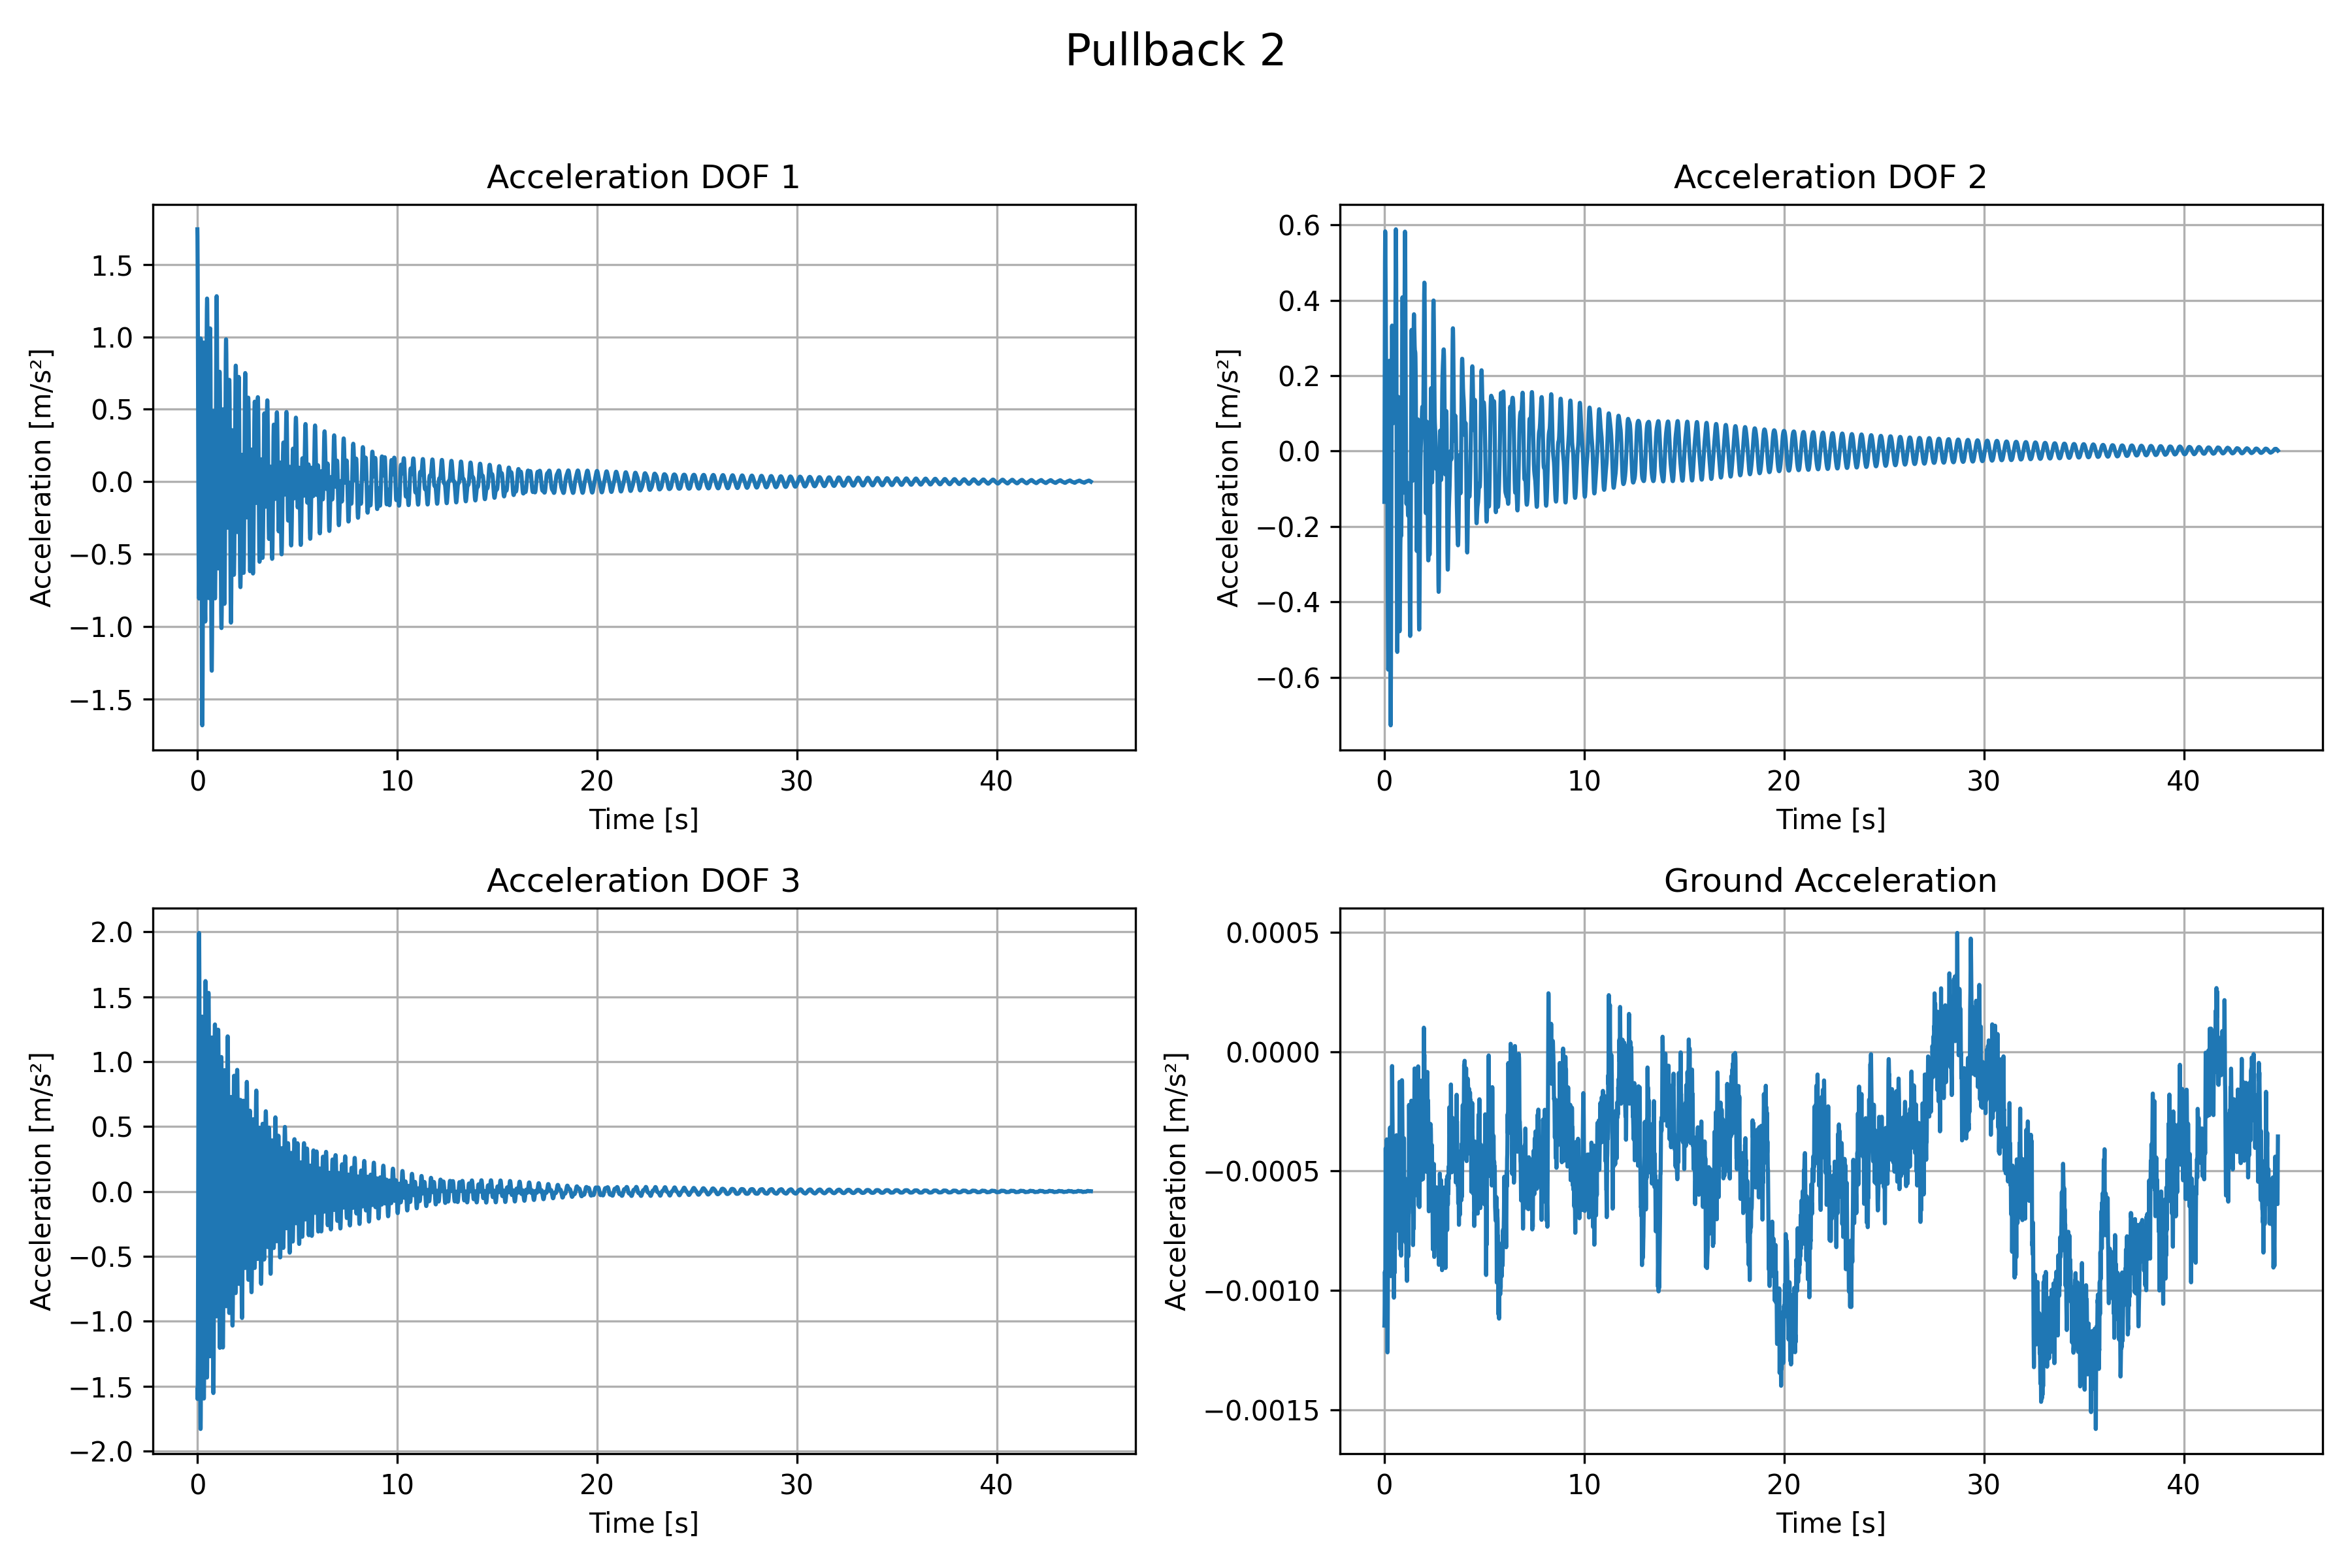
\includegraphics[width=\textwidth]{GRAFICOS/Pullback_2.png}
    \caption{Acceleration response of each DOF and ground during Pullback 2.}
    \label{fig:pullback_signal}
\end{figure}

To identify the dominant frequencies excited during the free vibration, the Fast Fourier Transform (FFT) was computed for each DOF. The results are presented in Figure~\ref{fig:fft_pullback}, where three distinct peaks can be observed for each signal, corresponding to the natural frequencies of the MDOF system.

\begin{figure}[H]
    \centering
    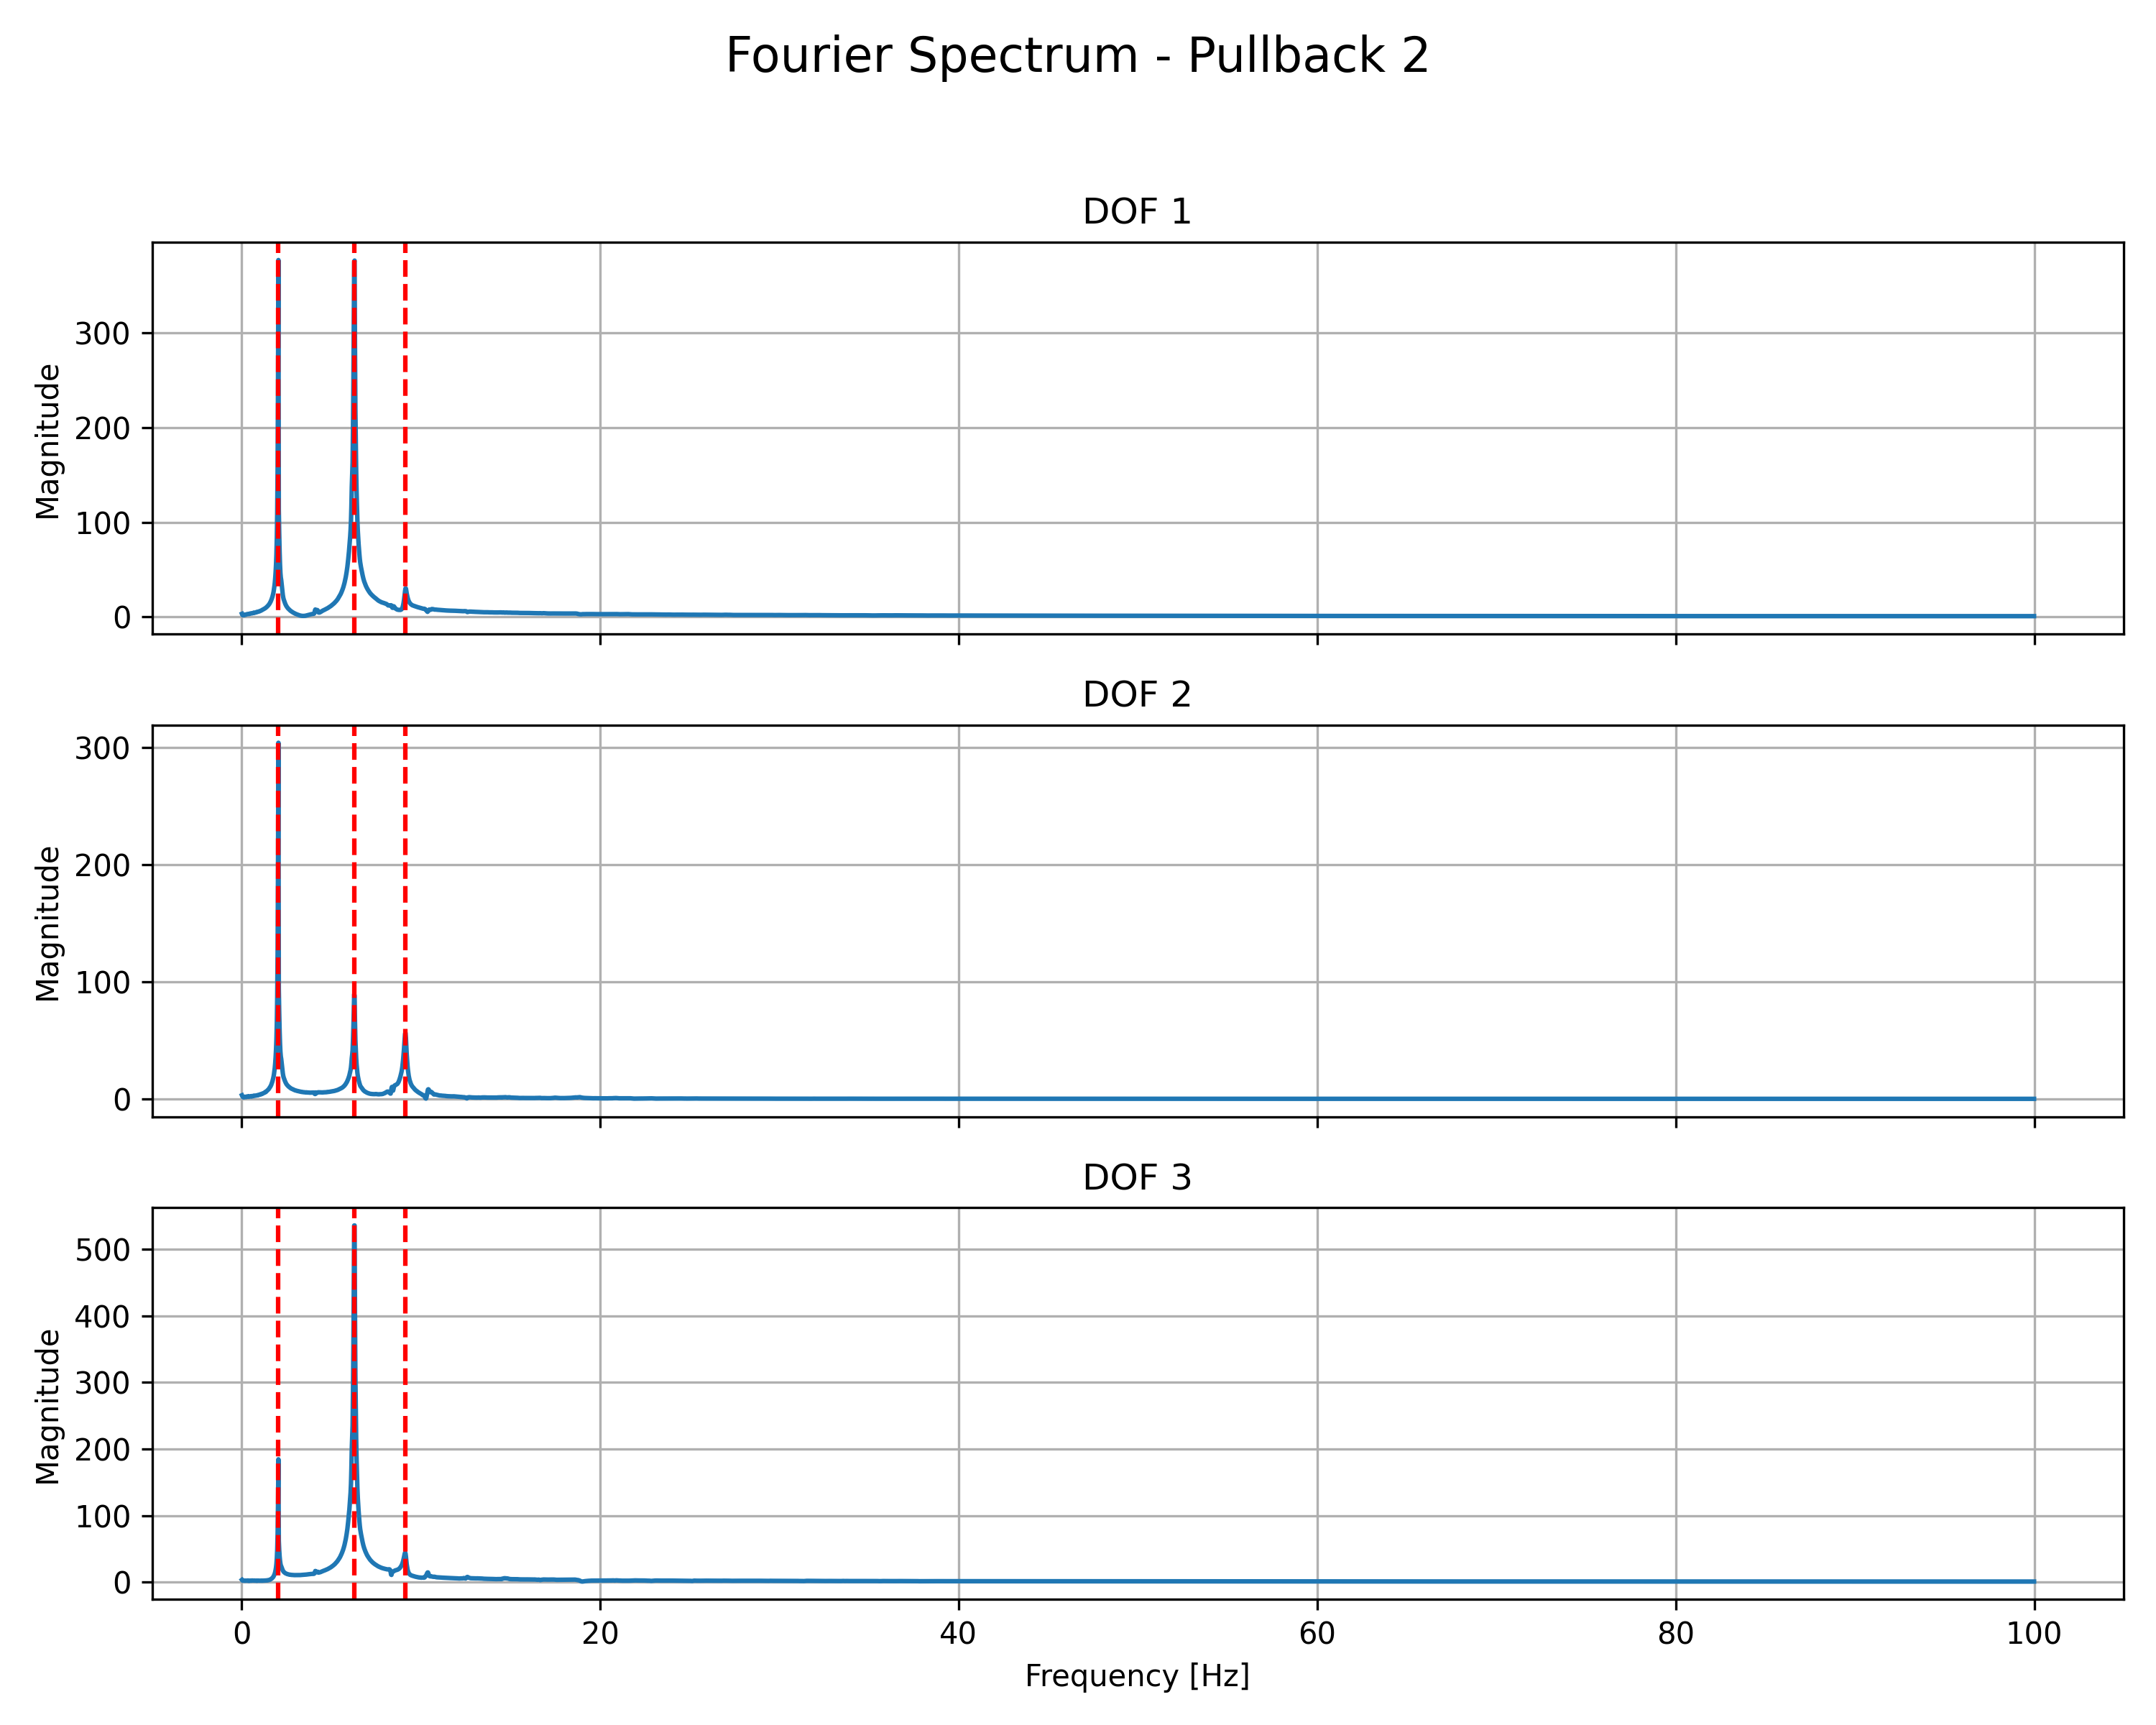
\includegraphics[width=0.9\textwidth]{GRAFICOS/Fourier_Pullback_2.png}
    \caption{Fourier spectrum of Pullback 2 for each DOF. Vertical dashed lines indicate the identified natural frequencies.}
    \label{fig:fft_pullback}
\end{figure}

The dominant frequencies identified from the FFT for each degree of freedom are:

\begin{itemize}
    \item \textbf{DOF 1:} 2.06 Hz, 6.31 Hz, 9.15 Hz
    \item \textbf{DOF 2:} 2.06 Hz, 6.28 Hz, 9.15 Hz
    \item \textbf{DOF 3:} 2.06 Hz, 6.31 Hz, 9.12 Hz
\end{itemize}

Using the decay of successive peaks in the time-domain response, the logarithmic decrement was applied to estimate the damping ratio $\zeta$. The damped natural period $T_d$ was calculated from the inverse of each dominant frequency. Table~\ref{tab:ld_results} summarizes the estimated values:

\begin{table}[H]
    \centering
    \begin{tabular}{lccc}
        \toprule
        \textbf{Mode} & $f_n$ (Hz) & $T_d$ (s) & $\zeta$ \\
        \midrule
        Mode 1 & 2.06 & 0.485 & 0.0114 \\
        Mode 2 & 6.30 & 0.159 & 0.0114 \\
        Mode 3 & 9.14 & 0.109 & 0.0114 \\
        \bottomrule
    \end{tabular}
    \caption{Natural frequencies, damped periods, and damping ratio estimated from Pullback 2.}
    \label{tab:ld_results}
\end{table}

As shown in the table, the structure exhibits three well-defined natural frequencies, with low damping ratios across all modes. These results confirm that the system behaves as a lightly damped MDOF structure. The consistent exponential decay and frequency peaks support the validity of the linear model used for modal analysis.

\subsection*{Comparison between Theoretical and Experimental Frequencies}

The natural frequencies obtained experimentally from the pull-back test (Pullback 2) were compared with the theoretical values computed from the analytical model of the MDOF system.

Table~\ref{tab:comparison_frequencies} summarizes the theoretical and experimental frequencies for the first three modes, along with the absolute difference and the relative error percentage.

\begin{table}[H]
    \centering
    \begin{tabular}{ccccc}
        \toprule
        \textbf{Mode} & \textbf{Theoretical $f_n$ [Hz]} & \textbf{Experimental $f_n$ [Hz]} & \textbf{Error [\%]} \\
        \midrule
        Mode 1 & 2.24 & 2.06  & 8.04\% \\
        Mode 2 & 6.04 & 6.30  & 4.30\% \\
        Mode 3 & 8.84 & 9.14  & 3.39\% \\
        \bottomrule
    \end{tabular}
    \caption{Comparison between theoretical and experimental natural frequencies.}
    \label{tab:comparison_frequencies}
\end{table}

As seen in Table~\ref{tab:comparison_frequencies}, the relative error between theoretical and experimental frequencies is below 9\% in all modes, which is considered acceptable given the assumptions made in the analytical model (e.g., ideal boundary conditions, perfectly linear behavior, simplified stiffness estimation). The experimental values tend to be slightly lower in the first mode and slightly higher in the higher modes, which may be due to non-idealities such as damping, assembly imperfections, or mass distribution effects.

\subsection*{Test with harmonic vibrations}

For this section, a comparison was made between the theoretical and experimental modes of vibrations of the strcuture when resonance occurs.

\begin{figure}[H]
    \centering
    \begin{subfigure}[b]{0.3\textwidth}
        \centering
        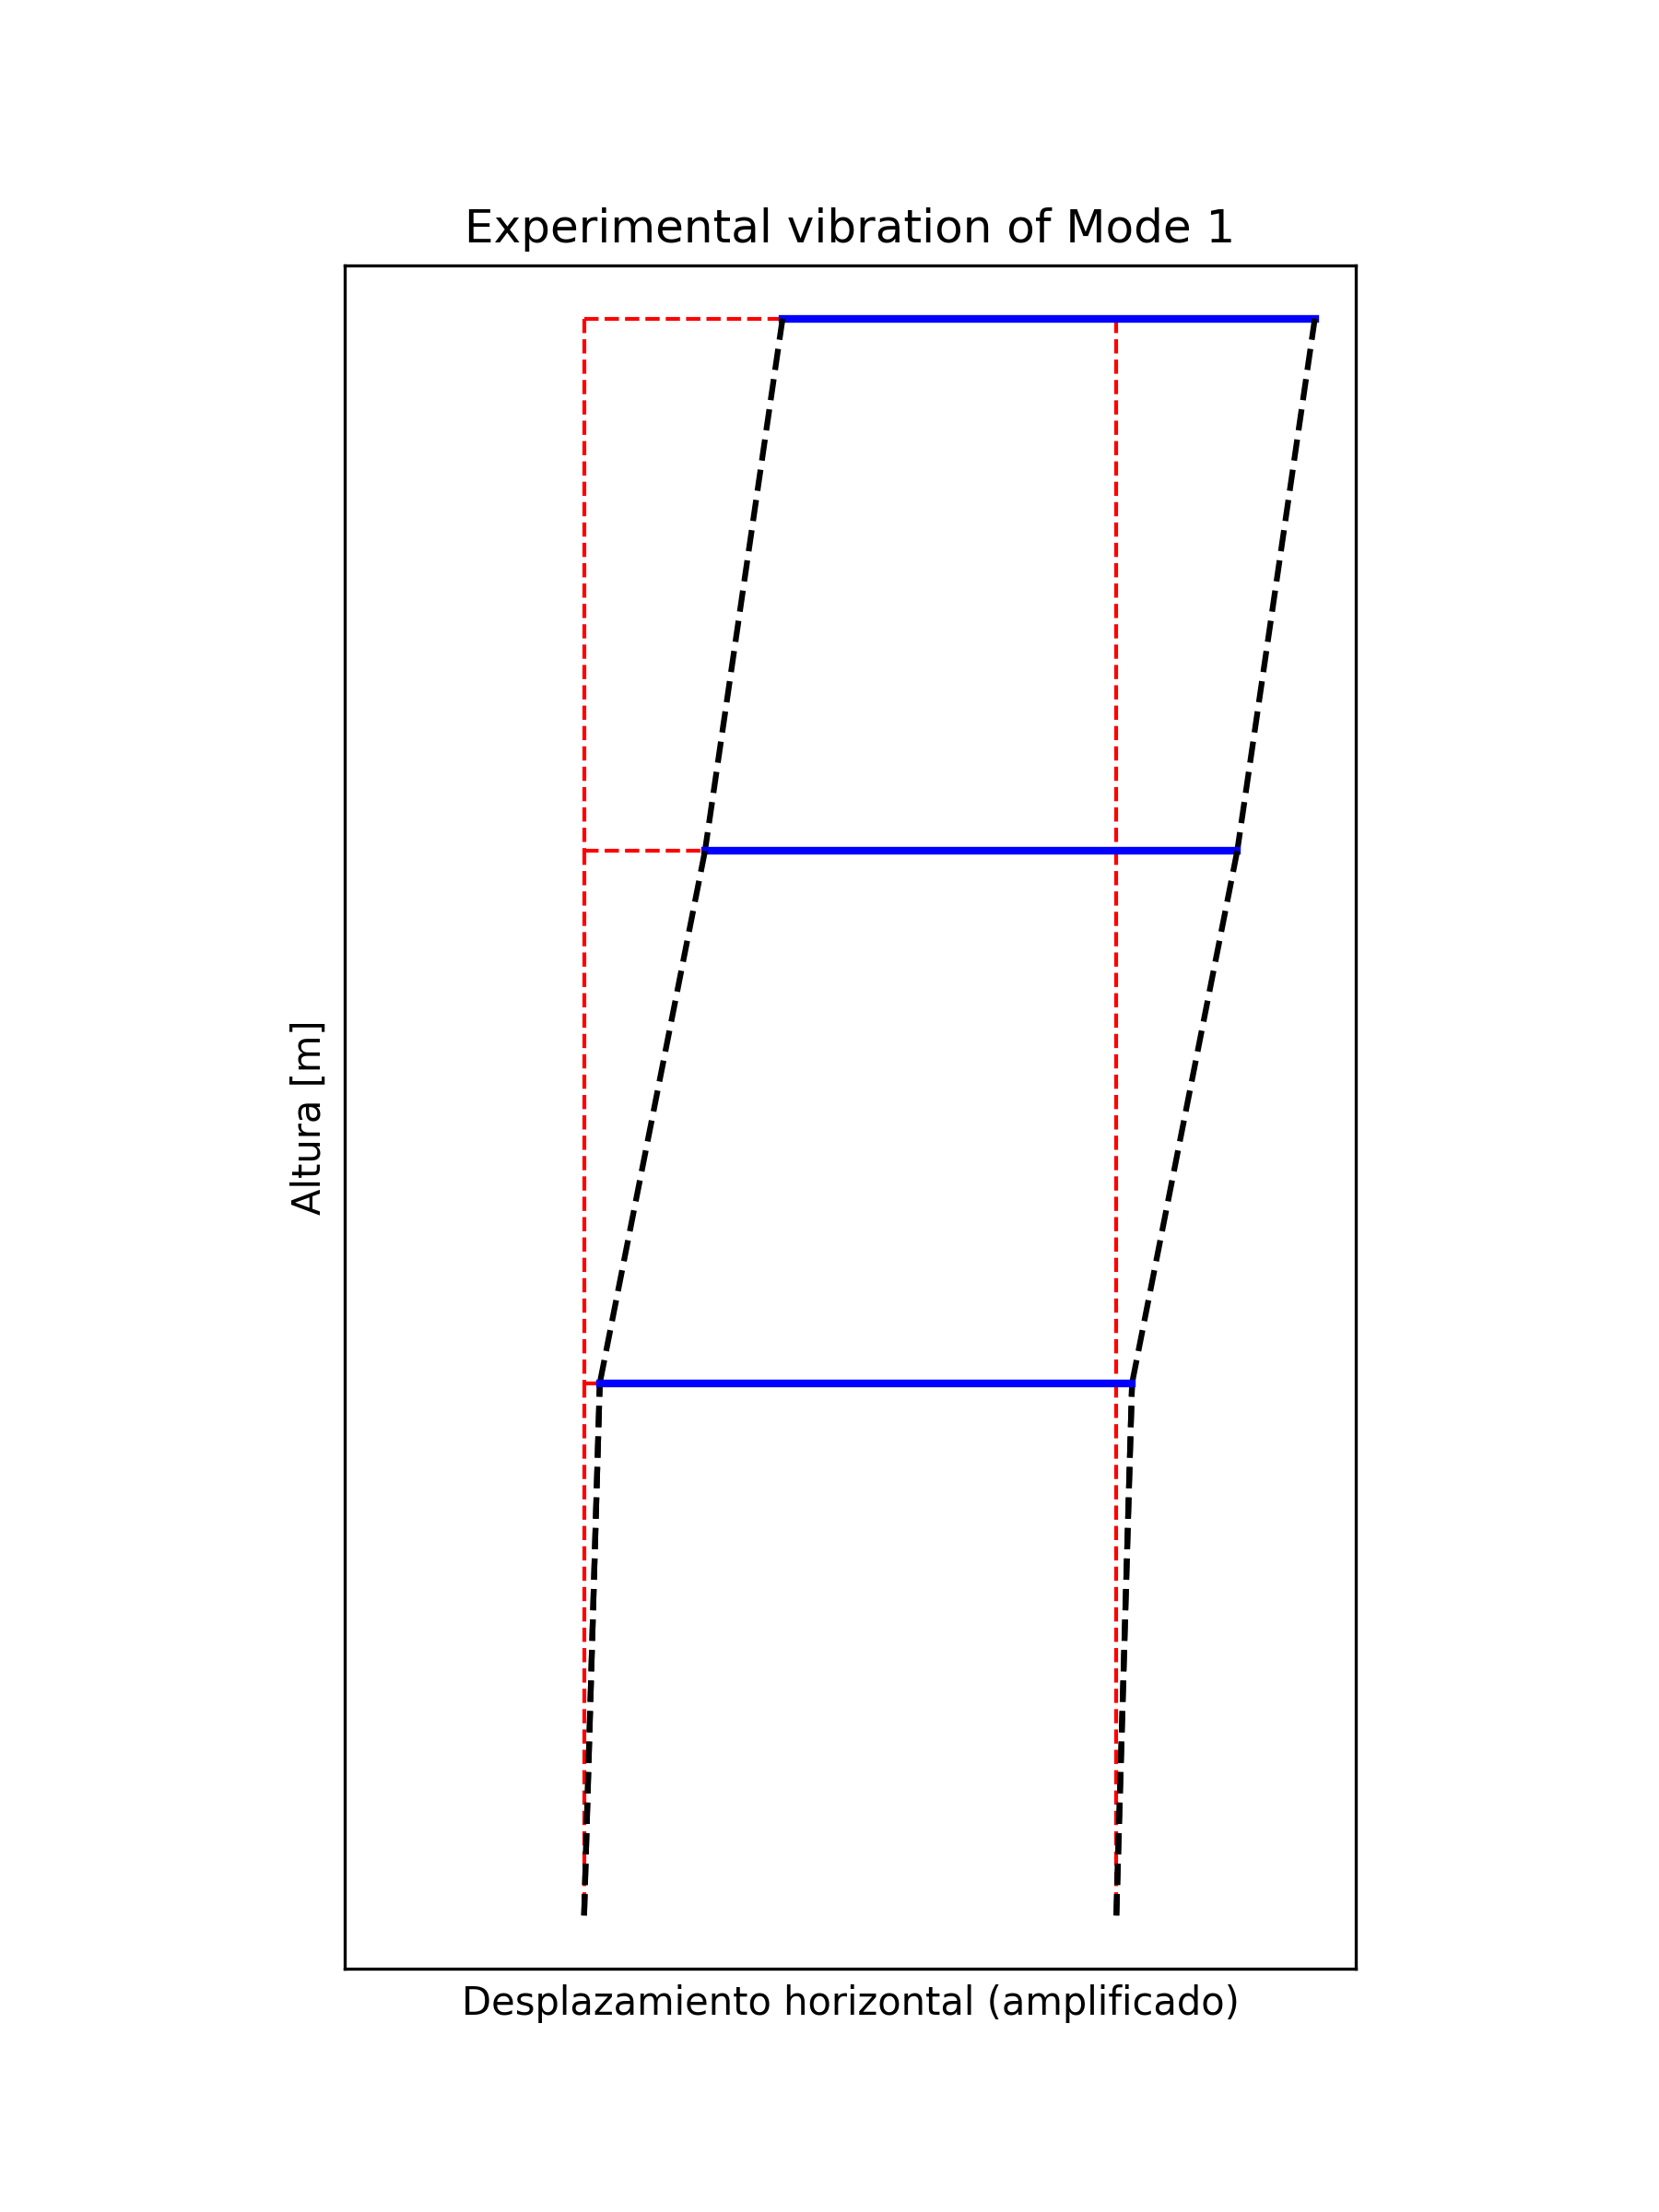
\includegraphics[width=\textwidth]{GRAFICOS/Modo_Experimental_Estructura_Sismico_1.png}
        \caption{VIbration Mode 1}
        \label{fig:modo1}
    \end{subfigure}
    \hfill
    \begin{subfigure}[b]{0.3\textwidth}
        \centering
        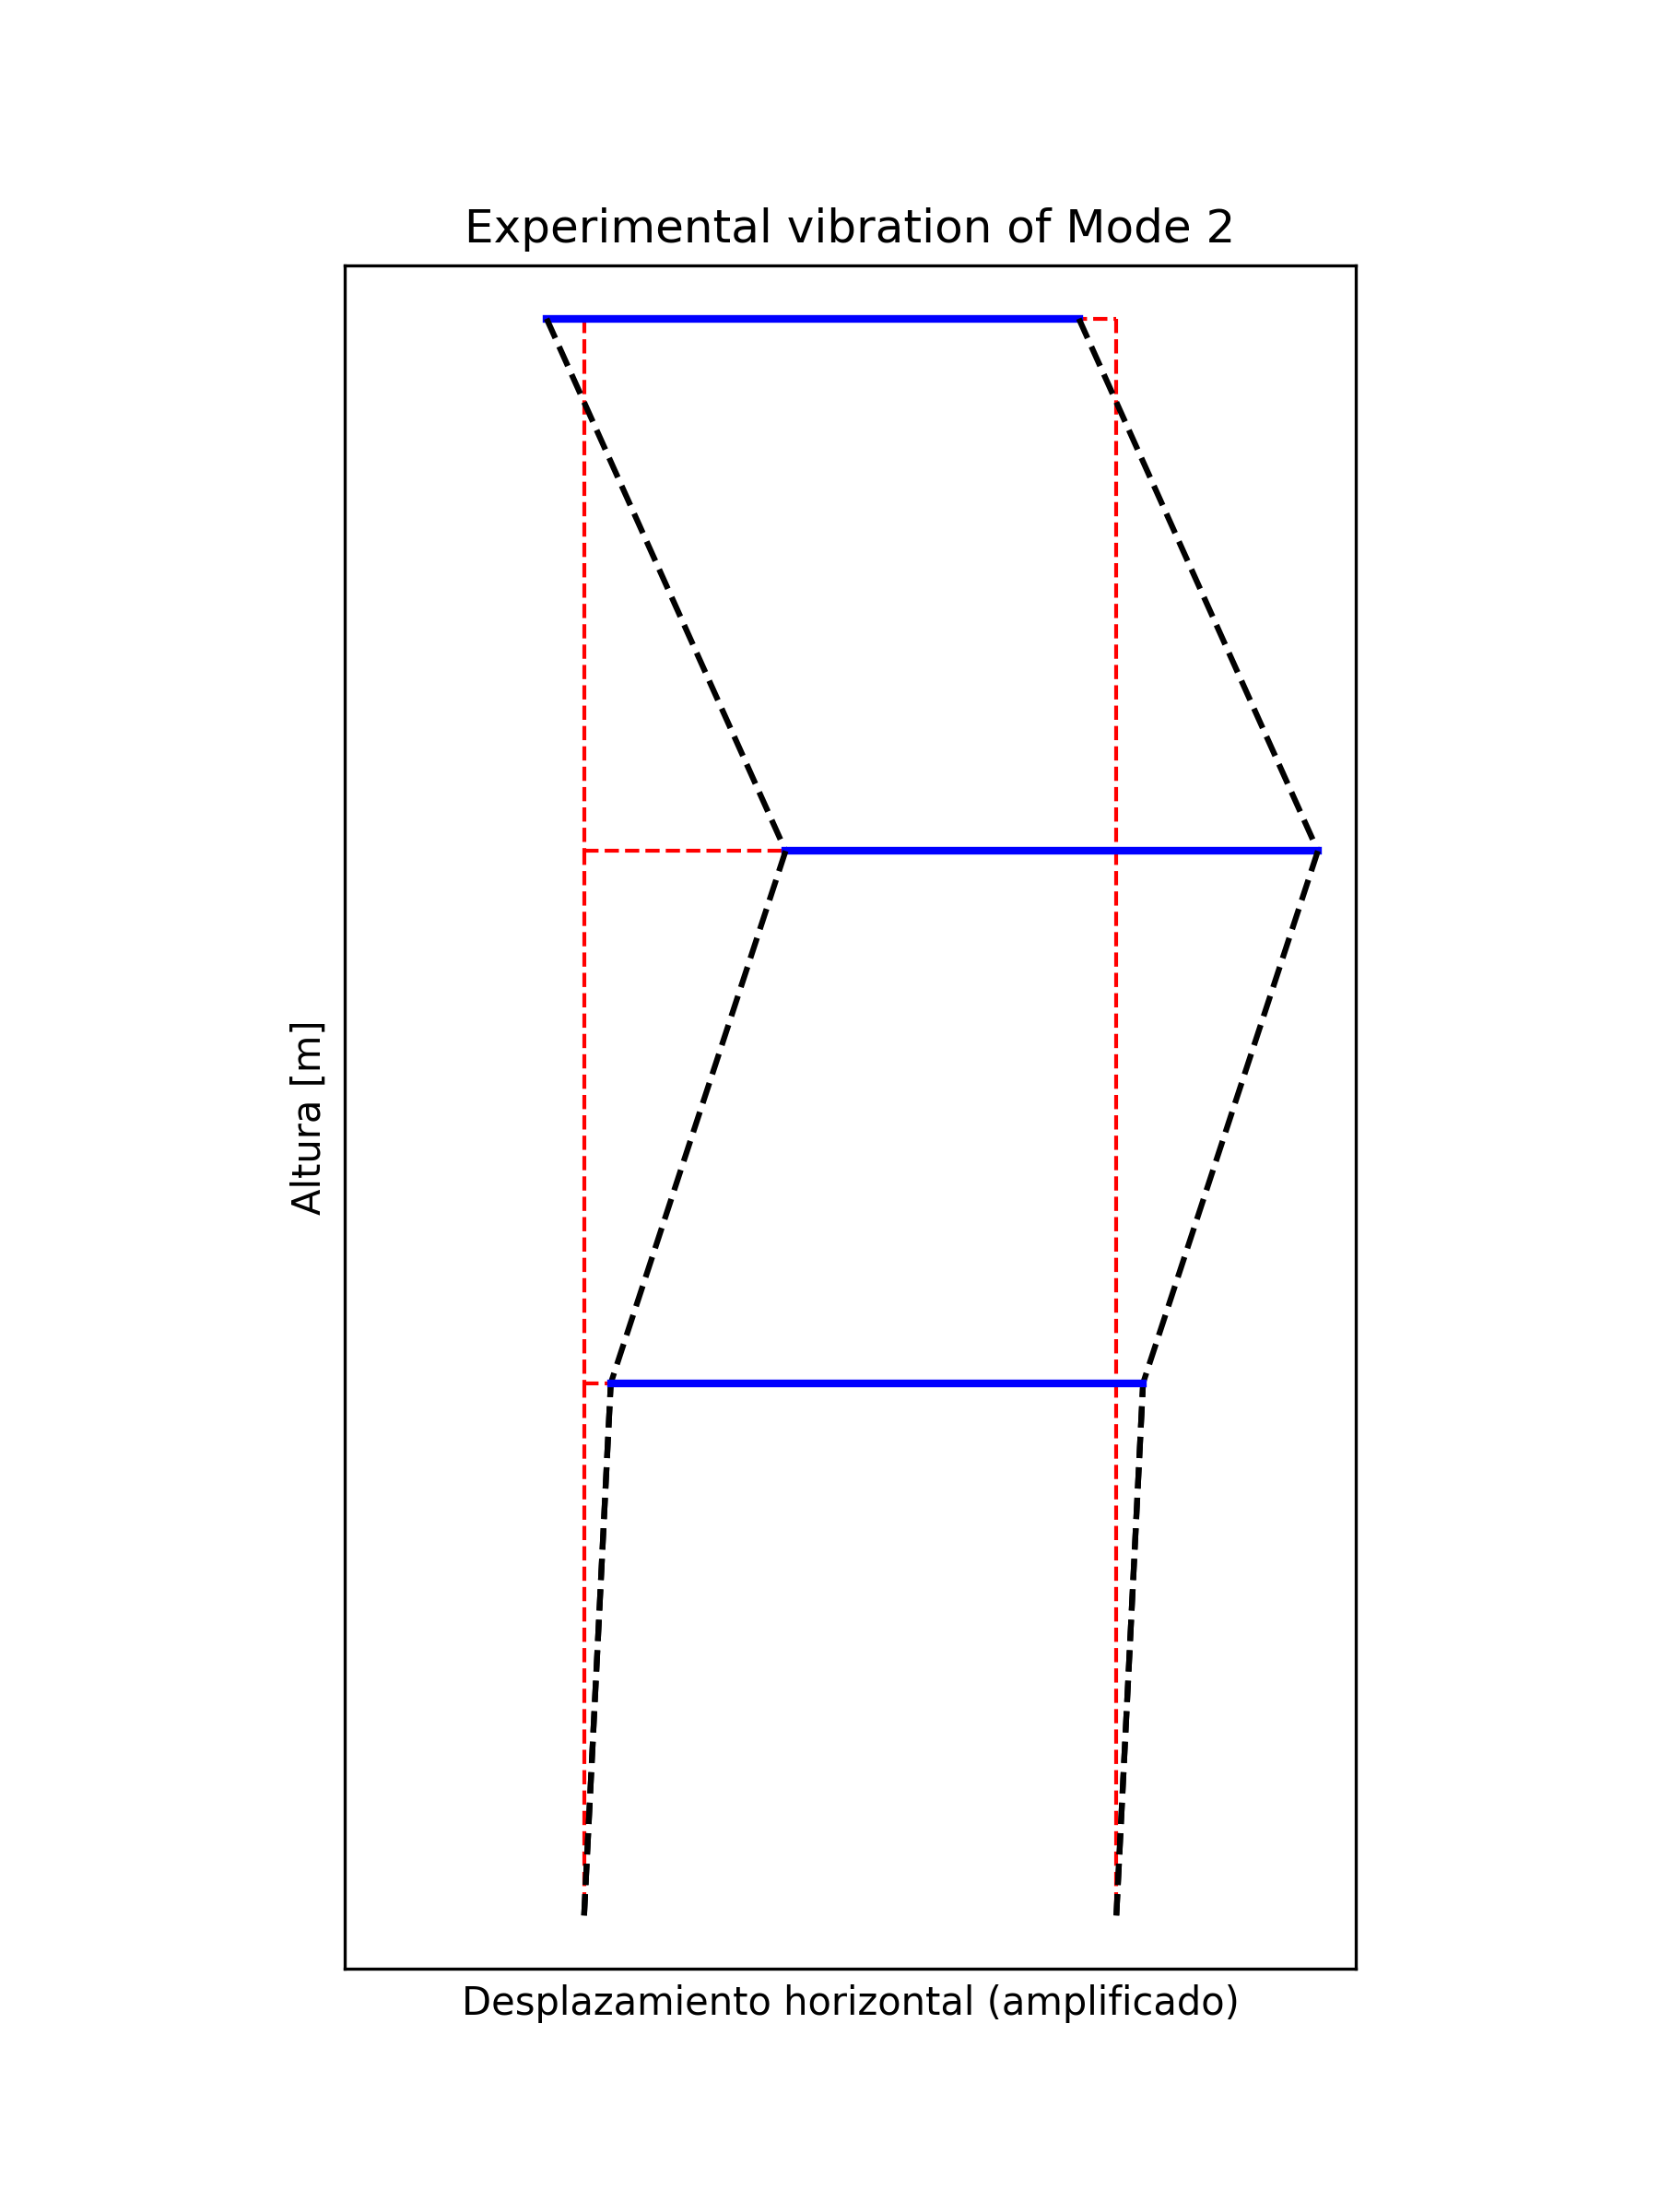
\includegraphics[width=\textwidth]{GRAFICOS/Modo_Experimental_Estructura_Sismico_2.png}
        \caption{Vibration Mode 2}
        \label{fig:modo2}
    \end{subfigure}
    \hfill
    \begin{subfigure}[b]{0.3\textwidth}
        \centering
        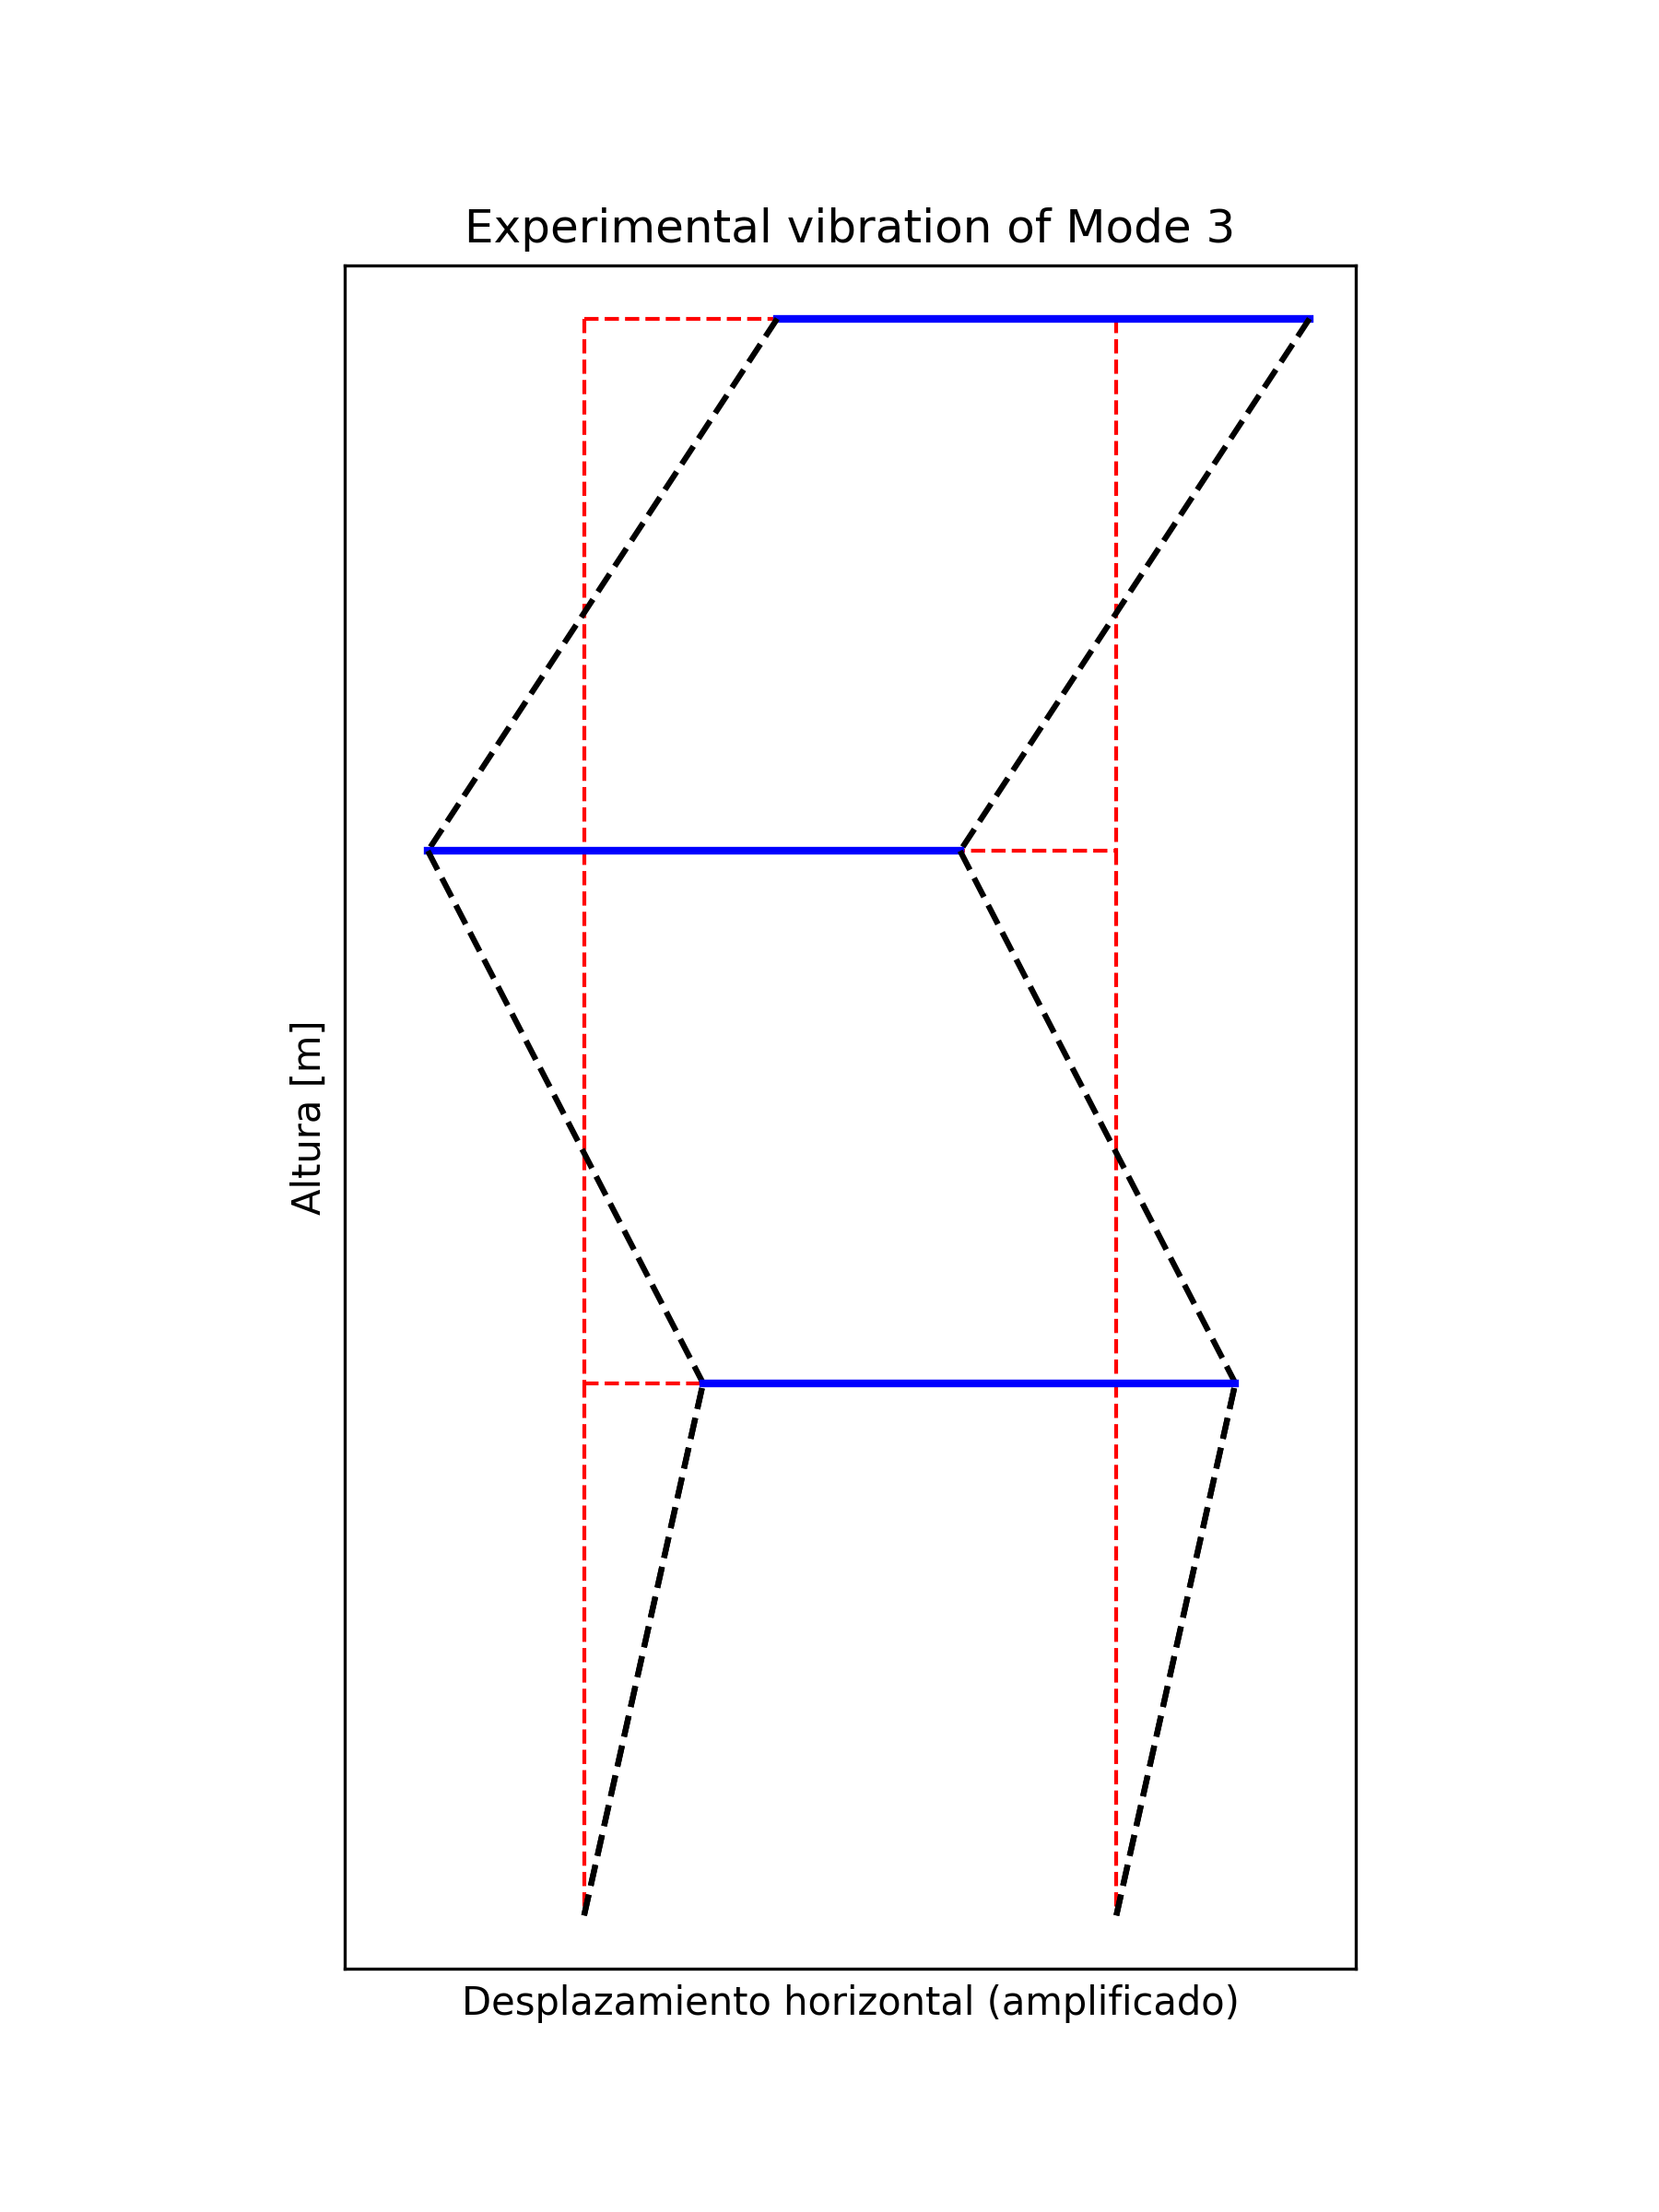
\includegraphics[width=\textwidth]{GRAFICOS/Modo_Experimental_Estructura_Sismico_3.png}
        \caption{Vibration Mode 3}
        \label{fig:modo3}
    \end{subfigure}
    \caption{Experimental vibration modes of the structure during resonance in harmonic excitation.}
    \label{fig:modos_exp}
\end{figure}

\begin{table}[H]
\centering
\begin{minipage}{0.45\textwidth}
    \centering
    \caption{Natural experimental frequencies of the structure}
    \begin{tabular}{c|c}
        \hline
        Mode & $f_n$ [Hz] \\
        \hline
        1 & 2.06 \\
        2 & 6.3 \\
        3 & 9.14 \\
        \hline
    \end{tabular}
    \label{tab:frecuencias}
\end{minipage}\hfill
\begin{minipage}{0.53\textwidth}
    \centering
    \caption{Normalized experimental mode shapes of the structure}
    \begin{tabular}{c|ccc}
        \hline
        Mode & Floor 1 & Floor 2 & Floor 3 \\
        \hline
        1 & 0.10 & 0.76 & 1.24 \\
        2 & 0.17 & 1.26 & -0.23 \\
        3 & 0.75 & -0.98 & 1.21 \\
        \hline
    \end{tabular}
    \label{tab:modos}
\end{minipage}
\end{table}

\begin{table}[H]
\centering
\caption{Normalized theoretical modes of the structure}
\begin{tabular}{c|ccc}
\hline
Mode & Floor 1& Floor 2 & Floor 3 \\
\hline
1 & 0.57 & 1.00 & 1.24 \\
2 & 0.36 & 0.11 & -0.30 \\
3 & 0.07 & -0.12 & 0.06 \\
\hline
\end{tabular}
\label{tab:normalized_modes_theoretical_swapped}
\end{table}

As Table \ref{tab:frecuencias}, \ref{tab:modos} and \ref{tab:normalized_modes_theoretical_swapped} shows, some differences are observed in both the frequencies and the mode shapes. These discrepancies can be attributed to factors such as model simplifications, experimental noise, or limitations in capturing the full dynamic behavior of the structure. Overall, the results highlight the effectiveness of the experimental approach while also indicating areas where further refinement of the model or the testing procedures may be beneficial.

Despite these differences, the vibration modes plotted were in accordance with the theoretical modes, confirming the expected behavior of the structure under harmonic excitation.

\newpage

\section*{Sismic Response Analysis}

In this section, the numerical siesmic response was obteined using the Newmark's method. This analysis was performed for two types of earthquakes, the Concepcion and Kobe earthquakes, which were scaled to match the maximum acceleration of the structure. The results were compared with the experimental data obtained from the shaking table tests.

\subsection*{Concepcion Earthquake}

\begin{figure}[H]
    \centering
    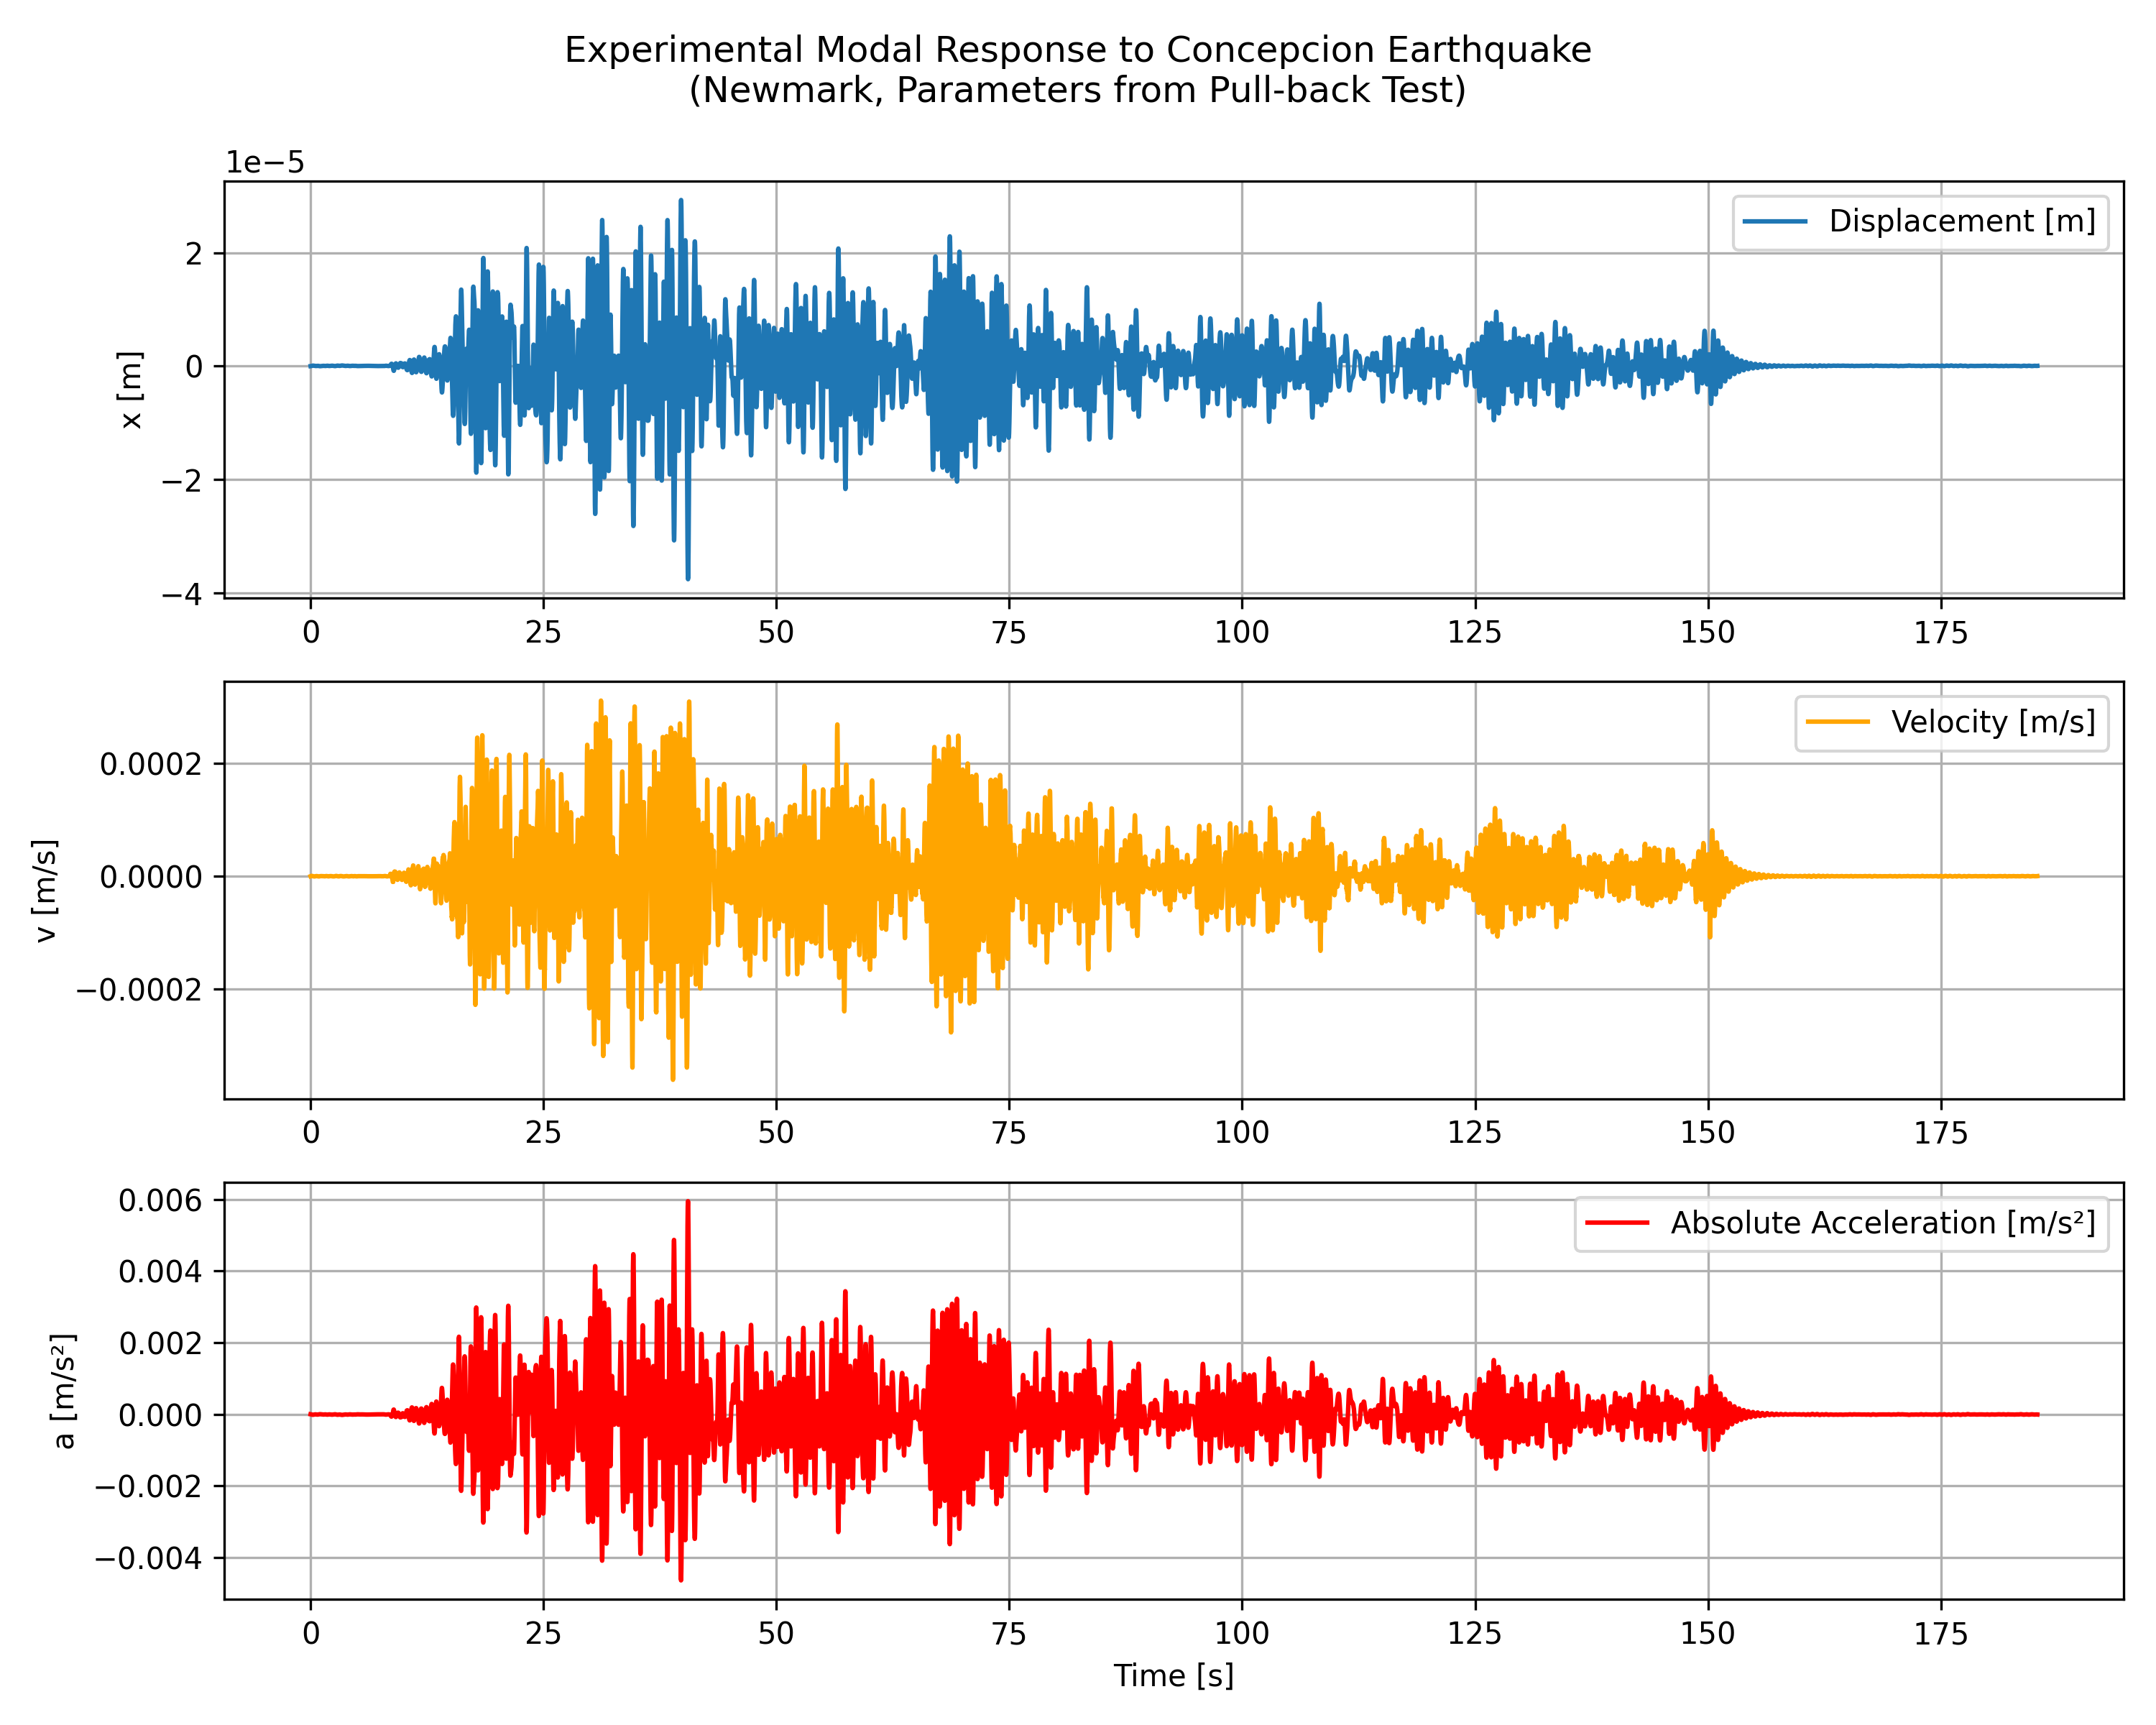
\includegraphics[width=0.8\textwidth]{GRAFICOS/Experimental_Response_Concepcion.png}
    \caption{Numerical response of the structure during the Concepción earthquake.}
    \label{fig:concepcion_acceleration}
\end{figure}

\subsection*{Kobe Earthquake}

\begin{figure}[H]
    \centering
    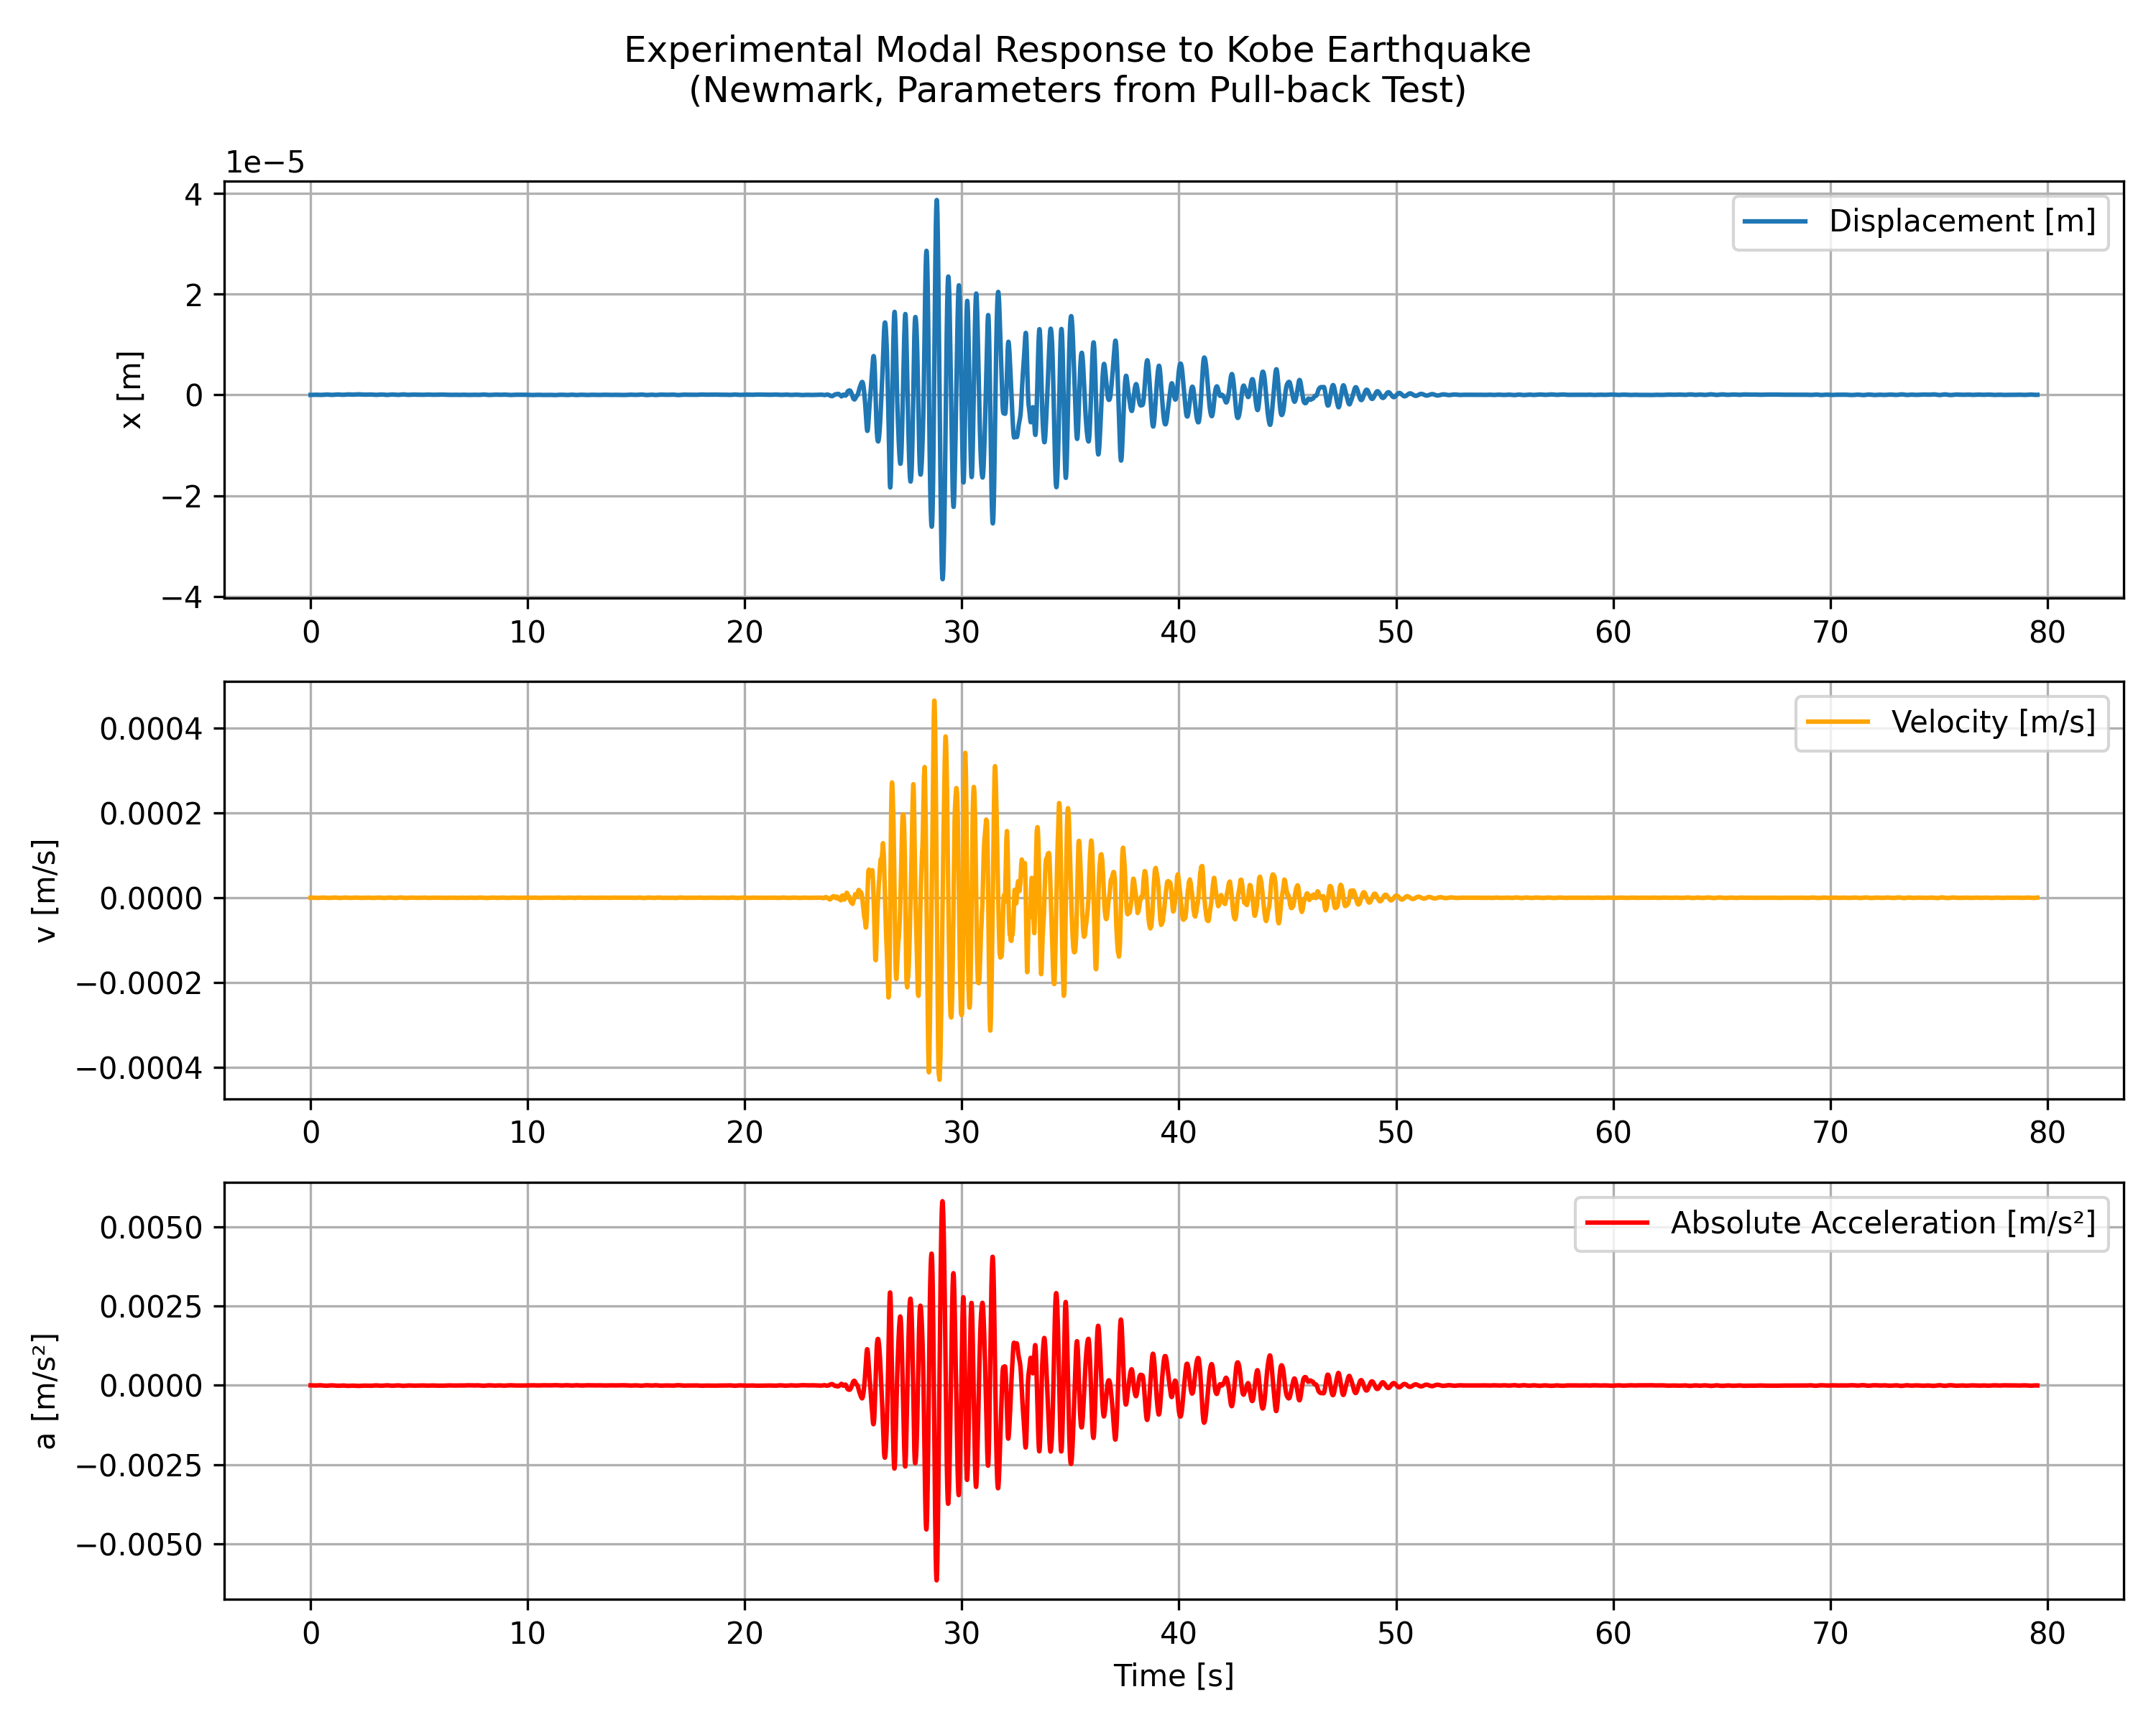
\includegraphics[width=0.8\textwidth]{GRAFICOS/Experimental_Response_Kobe.png}
    \caption{Numerical response of the structure during the Kobe earthquake.}
    \label{fig:kobe_acceleration}
\end{figure}

The simulated seismic responses of the structure to the Concepción and Kobe earthquakes, obtained using the experimentally identified first mode and the Newmark method, illustrate how the dynamic behavior is governed by both the characteristics of the ground motion and the modal properties of the system. The Concepción earthquake generates a response with greater amplitude and longer duration compared to the Kobe earthquake, reflecting its higher energy and extended shaking. In both cases, the system’s response closely follows that of a single-degree-of-freedom oscillator, dominated by the first mode, and the computed displacements and accelerations remain within the expected range for a lightly damped laboratory structure. Any minor differences in response details can be attributed to the distinct frequency content of each seismic input, experimental uncertainties, and the inherent simplifications of the SDOF approximation, yet overall, the simulations show good agreement with theoretical expectations and validate the experimental modal identification.

\newpage
\section*{Conclusions}

The comparison between theoretical and experimental results demonstrates strong agreement for the fundamental dynamic properties of the structure. Both analytical calculations and experimental tests, including pull-back and harmonic excitation, yield natural frequencies and mode shapes that are closely matched for the first mode, with relative errors under 9\%. While the first mode is consistently observed in all tests, higher-frequency modes are more challenging to detect and show greater discrepancies due to limitations in excitation methods, measurement noise, and model simplifications. The use of frequency domain analysis, such as FFT, proved especially valuable for identifying these higher modes and for contrasting the dynamic response under different testing conditions.

Differences between theoretical predictions and experimental findings can largely be attributed to modeling assumptions, sensor placement inaccuracies, and the presence of experimental noise. Refining the analytical model to better represent boundary conditions, mass distribution, and damping could help reduce these discrepancies. Additionally, advanced excitation techniques and signal processing methods may further enhance the identification of high-frequency modes in future work. Overall, the laboratory validated key concepts from lectures such as modal superposition, resonance, and the role of mass, stiffness, and damping through empirical results. All employed routines and Python scripts are included in the \href{https://github.com/LukasWolff2002/LAB_2_DYNAMICS}{GitHub Repository}.


\end{document}